
%\documentclass[mathserif]{beamer}
\documentclass[handout]{beamer}
%\usetheme{Goettingen}
%\usetheme{Warsaw}
\usetheme{Singapore}



%\usetheme{Frankfurt}
%\usetheme{Copenhagen}
%\usetheme{Szeged}
%\usetheme{Montpellier}
%\usetheme{CambridgeUS}
%\usecolortheme{}
%\setbeamercovered{transparent}
\usepackage[english, activeacute]{babel}
\usepackage[utf8]{inputenc}
\usepackage{amsmath, amssymb}
\usepackage{dsfont}
\usepackage{graphics}
\usepackage{cases}
\usepackage{graphicx}
\usepackage{pgf}
\usepackage{epsfig}
\usepackage{amssymb}
\usepackage{multirow}	
\usepackage{amstext}
\usepackage[ruled,vlined,lined]{algorithm2e}
\usepackage{amsmath}
\usepackage{epic}
\usepackage{epsfig}
\usepackage{fontenc}
\usepackage{framed,color}
\usepackage{palatino, url, multicol}
%\algsetup{indent=2em}
\newcommand{\factorial}{\ensuremath{\mbox{\sc Factorial}}}
\newcommand{\BIGOP}[1]{\mathop{\mathchoice%
{\raise-0.22em\hbox{\huge $#1$}}%
{\raise-0.05em\hbox{\Large $#1$}}{\hbox{\large $#1$}}{#1}}}
\newcommand{\bigtimes}{\BIGOP{\times}}
\vspace{-0.5cm}
\title{COMP321:  Sentiment Analysis}
\vspace{-0.5cm}
\author[Felipe Bravo Márquez]{\footnotesize
%\author{\footnotesize  
 \textcolor[rgb]{0.00,0.00,1.00}{Felipe Bravo-Marquez}} 
  
 
%\vspace{-0.3cm}
\institute{Department of Computer Science, University of Waikato }

\titlegraphic{
\includegraphics[scale=0.3]{pics/logo.pdf}}



\date{August, 2018}

\begin{document}
\begin{frame}
\titlepage


\end{frame}


\section{Introduction}





\begin{frame}{Social Media}
\begin{scriptsize}
\begin{itemize}
 \item Microblogging services are increasingly being adopted by people in order to access and publish information.  
 \item \textbf{Twitter}: Massively used Microblogging platform where users post messages limited to 280 characters referred to as \textbf{tweets}. 
 \item  Tweets can be used to convey  emotions,  opinions, and  stance.
\end{itemize}

\begin{figure}[htbp]
\begin{center}
\scalebox{0.7}{
\begin{tabular}{cc}

\includegraphics[scale=0.2]{pics/twitter.png} & 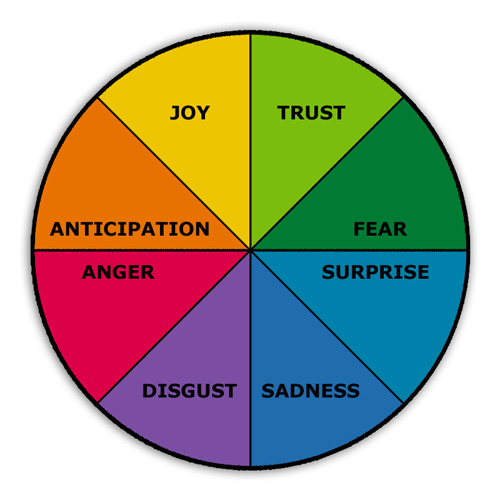
\includegraphics[scale=0.2]{pics/wheel_th.jpg} \\
\end{tabular}}
\end{center}
\end{figure}

\end{scriptsize}
\end{frame}



\begin{frame}{Sentiment Analysis and Social Media}
\begin{scriptsize}
\begin{itemize}
 \item Opinions are provided \textbf{freely and voluntarily} by the users in Twitter. 
 \item Analysing the sentiment underlying these opinions has important applications in product \textbf{marketing} and \textbf{politics}.
 
   \begin{figure}[h]
        	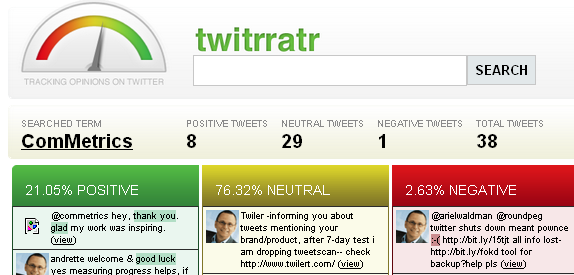
\includegraphics[scale = 0.6]{pics/tweetOpinions.png}
        \end{figure}
\end{itemize}
\end{scriptsize}




\end{frame}


\begin{frame}{Opinion Mining or Sentiment Analysis}
\begin{scriptsize}\begin{itemize}
 \item Application of \textbf{NLP} and \textbf{text mining} techniques to identify and extract subjective information from textual datasets.
\end{itemize}

\begin{block}{Main Problem: Message-level Polarity Classification (MPC)}
  \begin{enumerate}
   \item Automatically classify a tweet to classes \textcolor[rgb]{0.00,0.00,1.00}{\textbf{positive}}, \textcolor[rgb]{1.00,0.00,0.00}{\textbf{negative}}, or \textcolor[rgb]{0.00,1.00,0.00}{\textbf{neutral}}. 
   
     \begin{figure}[h]
        	
\includegraphics[scale = 0.15]{pics/sent.png}
        \end{figure}
   
   \item State-of-the-art solutions use \textbf{supervised} machine learning models trained from \textbf{manually} annotated examples \cite{Mohammad2013}.
  \end{enumerate} 
\end{block}

\end{scriptsize}

\end{frame}


\begin{frame}{Sentiment Classification via Supervised Learning}

\begin{figure}[h]
        	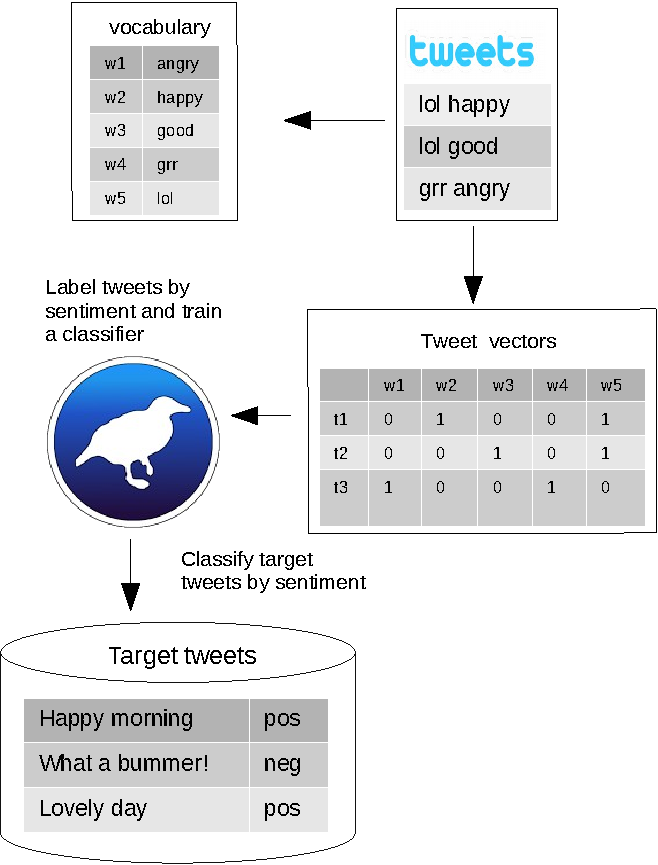
\includegraphics[scale = 0.5]{pics/bagOfwordsClassification.pdf}
        \end{figure}

\end{frame}




\begin{frame}{Supervised Learning: Support Vector Machines (SVMs)}
\begin{scriptsize}

\begin{itemize}


\item Idea: Find a hyperplane that separates the classes with the maximum margin (largest separation). 

     \begin{figure}[h]
        	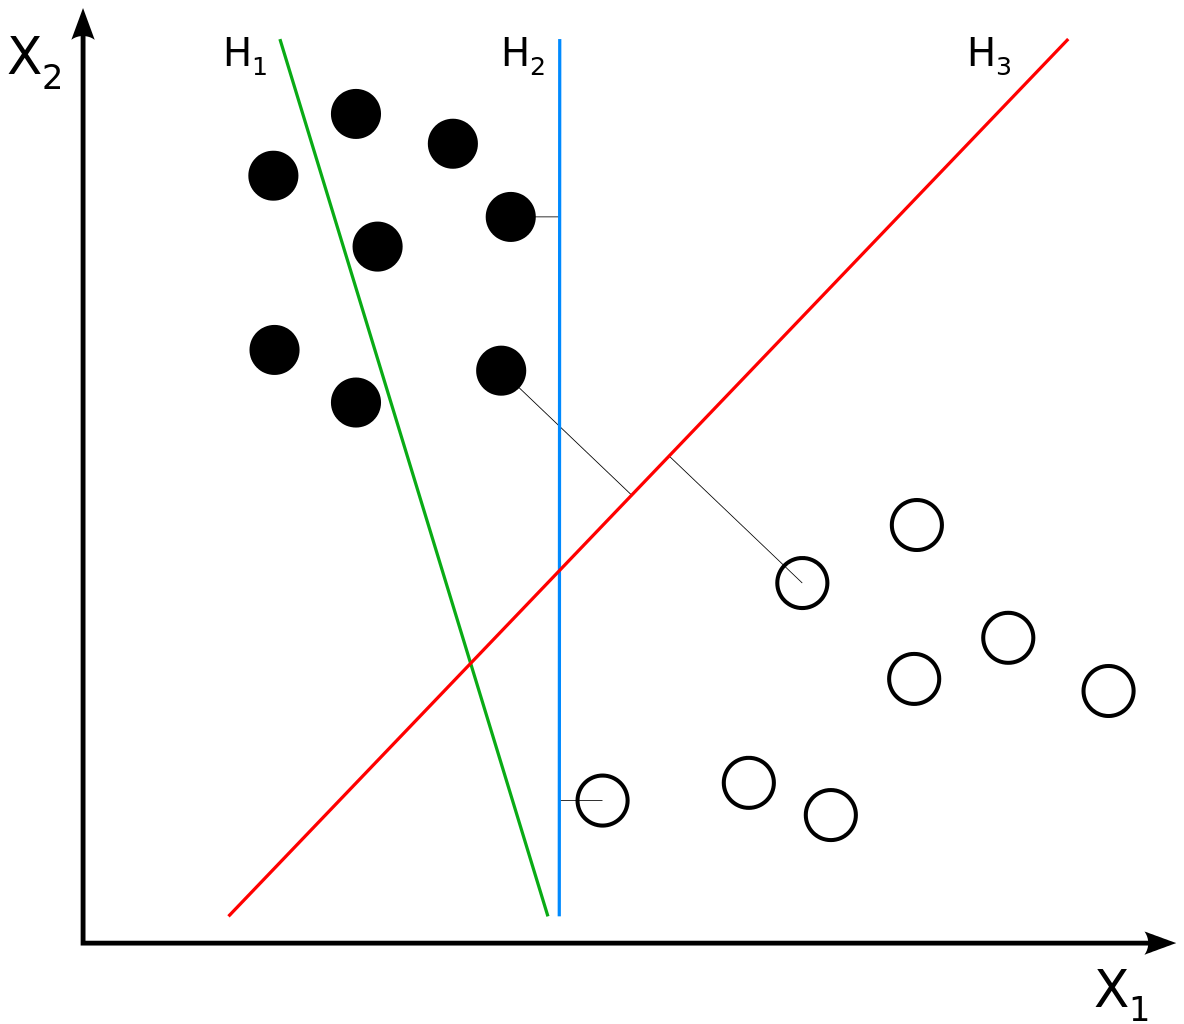
\includegraphics[scale = 0.15]{pics/SVM.png}
        \end{figure}

\item   
$H_3$ separates the classes with the maximum margin. 

\end{itemize}

\footnotemark{Image source: Wikipedia}       
   
\end{scriptsize}

\end{frame}


\begin{frame}{Related Tasks}

\begin{itemize}

  \item Stance Detection: detect if the author of a tweet is in favor, against or neutral regarding a given target (e.g., Donald Trump). 
   \item Irony/Sarcasm Detection: detecting sarcasm in tweets.
   \item Emotions classification: classify tweets according to multiple emotions (e.g., anger, fear, sadness, joy)
   \item  Infer emotion intensities (numerical values) in tweets (e.g., degree of anger).
   \item Affective\footnote{We will use the term ``\textbf{affect}'' to encompass sentiment, emotions, and other related concepts.} Lexicon Induction: classification of words into affective dimensions. 

\item Many of these probems have been evaluated in \textbf{SemEval} tasks.

\end{itemize}


\end{frame}



\begin{frame}{Challenges}
\begin{scriptsize}
  \begin{itemize}
   \item \textbf{Label sparsity (LS)}: manual annotation is \textbf{labour-intensive} and \textbf{time-consuming}. 
   \item \textbf{Concept drift}: the sentiment pattern can vary from one collection to another (domain-drift, temporal-drift).
 
 \item A classifier trained from tweets annotated for one domain will \textbf{not necessarily} work on another one! 
\item Trained models can become outdated over time.
  \end{itemize} 



\begin{block}{Examples of domain-Drift}
\begin{enumerate}
\item  For me the queue was pretty \textcolor[rgb]{0.00,0.00,1.00}{\textbf{small}} and it was only a 20 minute wait I think but was so worth it!!! :D @raynwise
\item Odd spatiality in Stuttgart. Hotel room is so  \textcolor[rgb]{1.00,0.00,0.00}{\textbf{small}} I can barely turn around but surroundings are inhumanly vast \& long under construction.
\end{enumerate}
\end{block}


\end{scriptsize}

\end{frame}

\begin{frame}{Label Sparsity}
\begin{scriptsize}

\begin{itemize}
\item A possible approach to \textbf{overcome} the sentiment-drift problem is to 
\textbf{constantly update} the sentiment classifier with \textbf{recent labelled data} \cite{bifet2010, Silva2011}.

\item The high arrival rates of social streams make the continuous acquirement of sentiment labels \textbf{infeasible} \cite{Silva2011, calais2011bias,Guerra2014}. 
\end{itemize}

\end{scriptsize}

\end{frame}


\begin{frame}{Approaches to overcome label sparsity}
\begin{scriptsize}
\begin{block}{Distant Supervision}
  \begin{itemize}
   \item Automatically \textbf{label} unlabelled data (\textbf{Twitter API}) using a heuristic method.
   \item \textbf{Emoticon-Annotation Approach (EAA)}: tweets with positive \textcolor[rgb]{0.00,0.00,1.00}{\textbf{:)}} or negative \textcolor[rgb]{1.00,0.00,0.00}{\textbf{:(}} emoticons are labelled according to the polarity indicated by the emoticon~\cite{Read2005}.
  \item The emoticon is \textbf{removed} from the content.
  \item The same approach has been extended using hashtags \#anger, and emojis.
\item Drawback: emoticons can induce noisy and incomplete information. Moreover they are not necessarily used in all domains (e.g., politics). 
\end{itemize} 
 
\end{block}

\begin{block}{Crowdsourcing}
  \begin{itemize}
\item Rely on services like \textbf{Amazon Mechanical Turk} or \textbf{Crowdflower} to ask the \textbf{crowds} to label a sample of the data on a demand-driven basis.
\item This can be expensive for online sentiment analysis (label sparsity problem). 
   \end{itemize} 
 
\end{block}

\end{scriptsize}

\end{frame}






\begin{frame}{Message-level Sentiment Classification}
\begin{scriptsize}
\begin{itemize}
\item In 2013, The Semantic Evaluation (SemEval) workshop organised the
``Sentiment Analysis in Twitter
task'' \cite{Semeval2013}.
 \item The task was divided into two sub-tasks: the expression
level and the message level. 
\item Expression-level: focused on determining
the sentiment polarity of a message according to a marked entity within
its content.
\item Message-level: the polarity has to be determined according to
the overall message.
\item  The organisers released training and testing datasets
for both tasks.
\cite{Semeval2013}
\end{itemize}
\end{scriptsize}
\end{frame}

%Tradi7onal: Curated sentiment dictionaries combined with either bag-of-words representa7ons (ignoring word order) or hand-designed nega7on features (aint gonna capture everything) 

% http://cs224d.stanford.edu/lectures/CS224d-Lecture1.pdf

\begin{frame}{The NRC System}
\begin{scriptsize}
\begin{itemize}
\item The team that achieved the highest performance in both
tasks among 44 teams was the \emph{NRC-Canada} team
\cite{Mohammad2013}.  
\item The team proposed a supervised approach using a linear SVM
classifier with the following hand-crafted features for representing tweets:
\begin{enumerate}
\begin{scriptsize}
\item  Word $n$-grams.
\item  Character $n$-grams. 
\item Part-of-speech tags.
\item Word clusters trained with the Brown clustering method~\cite{brown1992class}.
\item The number of elongated words (words with one character repeated more than two times).
\item The number of words with all characters in uppercase.
\item The presence of positive or negative emoticons.
\item The number of individual negations.
\item The number of contiguous sequences of dots, question marks and exclamation marks.
\item Features derived from polarity lexicons~\cite{Mohammad2013}. Two of these lexicons were generated using the PMI method from tweets annotated with hashtags and emoticons.
\end{scriptsize} 
\end{enumerate}
\end{itemize}
\end{scriptsize} 
\end{frame}




\begin{frame}{Feature Engineering and Deep Learning}
\begin{scriptsize}
\begin{itemize}
\item Designing the features of a winning NLP system requires a lot of domain-specific knowledge.
\item The NRC system was built before deep learning became popular in NLP.
\item Deep Learning systems on the other hand rely on representation learning to automatically learn good representations.
\item Large amounts of training data and faster multicore CPU/GPU machines are key in the success of deep learning. 
\item Neural networks and word embeddings play a key role in modern  architectures for NLP.
\end{itemize}
\end{scriptsize}
\end{frame}



\section{Affective Lexicon Induction}

\begin{frame}{The Twitter dialect}
\begin{scriptsize}
\begin{itemize}
\item An opinion lexicon is a lists of terms labelled by sentiment.
\item Lexicons are widely used resources for sentiment analysis
\item They are normally composed of positive and negative words such as \textcolor[rgb]{0.00,0.00,1.00}{\textbf{happy, wonderful}} and 
 \item The words used in Twitter include many abbreviations, acronyms, and misspelled words, e.g., \textbf{lol}, \textbf{omg}, \textbf{hahaha}, \textbf{\#hatemonday}.
\item This words are \textbf{not} covered by most popular lexicons.
\item The manual creation of a Twitter-oriented opinion lexicon is a \textbf{time-consuming} task.
\end{itemize}
\end{scriptsize}
\end{frame}






\begin{frame}{Automatic Lexicon Expansion}
\begin{scriptsize}
\begin{itemize}
\item Turney et.al proposed the PMI \textbf{semantic orientation} (PMI-SO) metric \cite{turney2003measuring}.
\item Point-wise mutual information \textbf{PMI}: Information-theoretic association metric between discrete variables.
\item PMI-SO: calculated as the difference between the \textbf{PMI} of the word with a positive and a negative seed word.

\begin{equation}
 \operatorname{PMI}(term_{1}, term_{2})= \log_{2} \left ( \frac{Pr(term_{1} \wedge term_{2})}{Pr(term_{1})Pr(term_{2})} \right )
\end{equation}

\begin{equation}\label{eq:so}
 \operatorname{SO}(word) = \operatorname{PMI}(word, ``excellent") - \operatorname{PMI}(word, ``poor")
\end{equation}

\item The PMI values are estimated by the number of \textbf{hits} returned by a search engine.

\item The resulting PMI-SO score is a numerical value whose \textbf{sign} represents the word's polarity.

\item The magnitude of the value represents the \textbf{sentiment intensity}. 


\end{itemize}
\end{scriptsize}
\end{frame}




\begin{frame}{Twitter lexicon expansion using PMI-SO}
\begin{scriptsize}
\begin{itemize}
\item Previous Twitter lexicon induction models compute the PMI-SO between \textbf{corpus words} and tweet-level sentiment \textbf{labels}. 
\item The tweets are \textbf{automatically} labelled to polarity classes using \textbf{distant supervision} \cite{Mohammad2013, Zhou2014} or \textbf{self-training} \cite{avaya2013}. 
\item  Distant supervision methods rely on strong \textbf{sentiment signals} found in the message such as \textbf{emoticons} \cite{Mohammad2013, Zhou2014} or \textbf{hashtags}  \cite{Mohammad2013} to label the messages.
\item  Tweets where these signals are not observed are \textbf{discarded}. 
\end{itemize}

\begin{table}[htbp]
\centering
\begin{tabular}{|l|l|}
\hline
positive & negative \\ \hline
:) & :( \\ 
:-) & :-( \\ 
:D & =( \\ 
=) & :'(   \\ \hline
\end{tabular}
\end{table} 


\end{scriptsize}
\end{frame}


\begin{frame}{Lexicon Induction with Distributional Vectors}
\begin{scriptsize}
\begin{itemize}
\item \textbf{Distributional Hypothesis} \cite{harris1954}: words occurring in the same \textbf{contexts} tend to have similar meanings.
\item Or equivalently: ``a word is characterized by the \textbf{company} it keeps".
\item \textbf{Distributional representations}: words are represented by \textbf{high-dimensional vectors} based on the context's where they occur. 

\end{itemize}
\end{scriptsize}
\end{frame}

\begin{frame}{Lexicon Induction with Distributional Vectors}
\begin{scriptsize}
\begin{enumerate}
\item Calculate word distributional vectors from a corpus of unlabelled tweets.
\item Label some training words with a seed lexicon.
\item Train a classifier on the seed words.
\item Use the classifier to induce the sentiment of all words from the corpus.
\end{enumerate}
\end{scriptsize}
\end{frame}

\begin{frame}{Word-context Matrices}
\begin{scriptsize}
\begin{itemize}
\item Distributional vectors are built from word-context matrices $M$. 
\item Each cell $(i,j)$ is a co-occurrence based association value between a \textbf{target word} $w_i$ and a \textbf{context} $c_j$ calculated  from a corpus of documents.
\item Contexts are commonly defined as windows of words surrounding $w_i$.
\item The window length $k$ is a parameter ( between 1 and 8 words on both the left and the right sides of $w_i$).
\item If the Vocabulary of the target words and context words is the same, $M$ has dimensionality $|\mathcal{V}| \times |\mathcal{V}|$.
\item Whereas shorter windows are likely to capture \textbf{syntactic information} (e.g, POS), longer windows are more likely to capture topical similarity \cite{goldberg2016primer, JurafskyBook}.
\end{itemize}

\end{scriptsize}
\end{frame}



\begin{frame}{Distributional Vectors with context windows of size 1}


\begin{figure}[htb]
	\centering
	 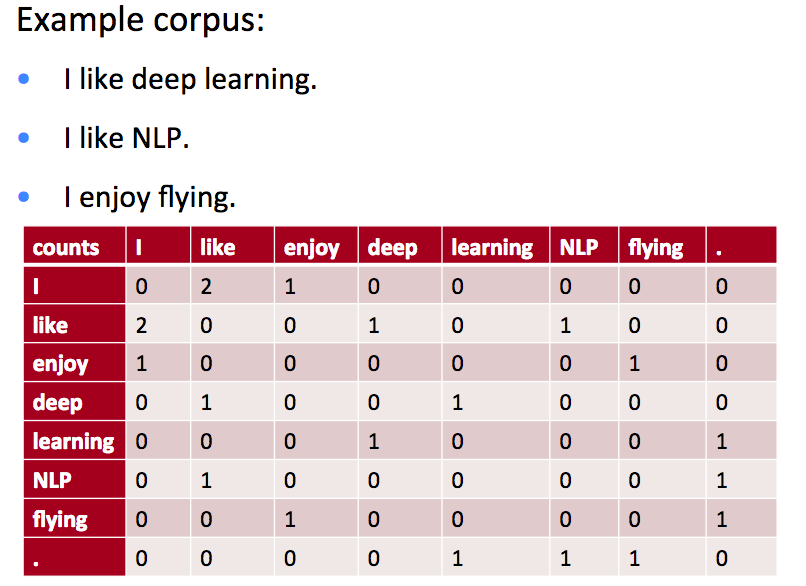
\includegraphics[scale=0.3]{pics/distributionalSocher.png}
\end{figure}


\footnotetext{Example taken from:    \url{http://cs224d.stanford.edu/lectures/CS224d-Lecture2.pdf}}
%\footnote{Source: \url{http://cs224d.stanford.edu/lectures/CS224d-Lecture2.pdf}}

\end{frame}



\begin{frame}{Word-context Matrices}
\begin{scriptsize}
The associations between words and contexts can be calculated using different approaches:
\begin{enumerate}
 \item Co-occurrence counts
\item Positive point-wise mutual information (PPMI)
\item The significance values of a paired t-test.  
\end{enumerate}

The most common of those according to \cite{JurafskyBook} is PPMI.

Distributional methods are also referred to as count-based methods.

\end{scriptsize}
\end{frame}



\begin{frame}{PPMI}
\begin{scriptsize}
\begin{itemize}
\item PPMI a filtered version of the traditional PMI measure in which negative values are set to zero:
\begin{equation}
 \operatorname{PPMI}(w, c)= \operatorname{max}(0,\operatorname{PMI}(w, c))
\end{equation}

\begin{equation}
 \operatorname{PPMI}(w,c)= \max \left (0, \log_{2} \left ( \frac{\operatorname{count}(w,c)\times |D|}{\operatorname{count}(w)\times \operatorname{count}(c)} \right )\right ). 
\end{equation}
\item  PMI calculates the log of the probability of word-context pairs occurring together over the probability of them being independent. 
\item Negative PMI values suggest that the pair co-occurs less often than chance. 
\item These estimates are unreliable unless the counts are calculated from very large corpora \cite{JurafskyBook}.
\item  PPMI corrects this problem by replacing negative values by zero. 
\end{itemize}
\end{scriptsize}
\end{frame}




\begin{frame}{Distributed Vectors or Word embeddings}
\begin{scriptsize}
\begin{itemize}

\item Count-based distributional vectors increase in size with vocabulary i.e., can have a very high dimensionality.

\item Explicitly storing the co-occurrence matrix can be memory-intensive. 

\item Some classification models don't scale well to high-dimensional data.

\item  The neural network community prefers using \textbf{distributed representations}\footnote{Idea: The meaning of the word is ``distributed'' over a combination of dimensions.} or \textbf{word embeddings}.

\item  Word \textbf{embeddings} are low-dimensional continuous dense word vectors trained from document corpora using \textbf{neural networks}.

\item They have become a crucial component of Neural Network architectures for NLP.


\end{itemize}
\end{scriptsize}
\end{frame}






\begin{frame}{Distributed Vectors or Word embeddings (2)}
\begin{scriptsize}
\begin{itemize}


\item They usually rely on an auxiliary predictive task (e.g., predict the following word).

\item The dimensions are not directly interpretable i.e., represent latent features of  the  word,  ``hopefully capturing useful syntactic and semantic properties''\cite{turian2010word}.

\item Most popular models are skip-gram \cite{Mikolov2013}, continuos bag-of-words \cite{Mikolov2013}, and Glove \cite{penningtonSM14}.

\item Word embeddings have shown to be more powerful than distributional approaches in many NLP tasks~\cite{baroni2014don}.

\item In \cite{amir2015SemEval}, they were used as \textbf{features} in a regression model for determining the association between Twitter words and \textbf{positive sentiment}. 

\end{itemize}
\end{scriptsize}
\end{frame}




\begin{frame}{Detour: Brief Introduction to Neural Networks}
\begin{scriptsize}
\begin{itemize}
\item Very popular machine learning models formed by units called \textbf{neurons}.
\item A neuron is a computational unit that has scalar inputs and outputs. 
\item  Each input has an associated weight $w$.
 \item The neuron multiplies each input by its weight, and then sums them (other functions such as \textbf{max} are also possible). 
\item It applies an activation function $g$ (usually non-linear) to the result, and passes it to its output.
\item Multiple layers can be stacked.
\end{itemize}


\end{scriptsize}
\end{frame}


\begin{frame}{Activation Functions}

\begin{scriptsize}
\begin{itemize}
\item The nonlinear activation function $g$ has a crucial role in the network's ability to represent complex functions. 
\item Without the nonlinearity in g, the neural network can only represent linear transformations of the input.
\end{itemize}


\end{scriptsize}

\begin{figure}[htb]
	\centering
	 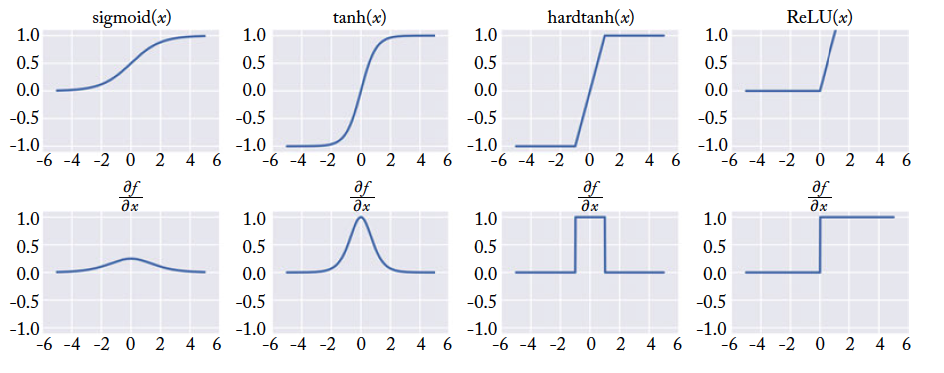
\includegraphics[scale=0.24]{pics/activations.png}
\end{figure}

\footnotetext{Source:\cite{goldberg2016primer}}

\end{frame}


\begin{frame}{Feedforward Network with two Layers}


\begin{figure}[htb]
	\centering
	 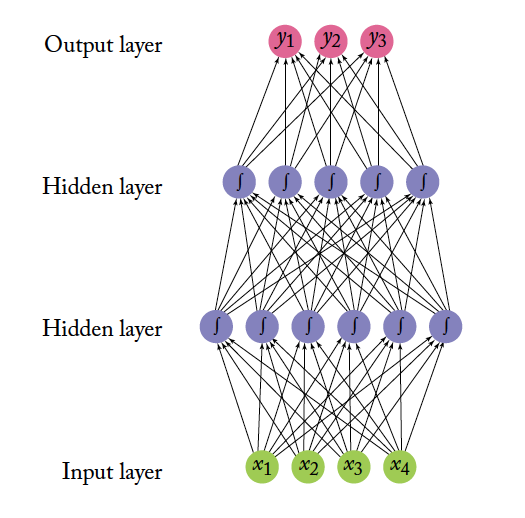
\includegraphics[scale=0.38]{pics/NN-example.png}
\end{figure}

\footnotetext{Source:\cite{goldberg2016primer}}

\end{frame}



\begin{frame}{Detour: Brief Introduction to Neural Networks}
\begin{scriptsize}
\begin{itemize}
\item The feedforward network from the picture is a stack of linear models separated by nonlinear functions.
\item The values of each row of neurons in the network can be thought of as a vector. 

\item The input layer is a 4-dimensional vector $(x)$, and the layer above it is a 6-dimensional vector $(h_1)$.
\item The fully connected layer can be thought of as a linear transformation from 4 dimensions to 6 dimensions. 
\item A fully connected layer implements a vector-matrix multiplication, $h=xW$.
\item The weight of the connection from the $i$-th neuron in the input row to the $j$-th neuron in the output row is $W_{[i,j]}$.
\item The values of $h$ are transformed by a nonlinear function $g$ that is applied to each value before being passed on as input to the next layer.

\end{itemize}


\end{scriptsize}
\end{frame}





\begin{frame}{Detour: Brief Introduction to Neural Networks}
\begin{scriptsize}
\begin{itemize}
\item The Multilayer Perceptron (MLP) from the figure can be written as the following mathematical function:
\begin{center}
\begin{equation}
\begin{split}
NN_{MLP2(x)} & =  y  \\
h^{1} &  = g^{1}(xW^{1}+b^{1}) \\
h^{2} &  = g^{2}(h^{1}W^{2}+b^{2}) \\
y &  = h^{2}W^{3}\\
y &  = (g^2(g^1(xW^{1}+b^{1})W^2+b^2))W^3.\\
\end{split}
\end{equation}
\end{center}
%NN_{MLP2(x)}  =  y \\
%h^{1} = g^{1}(xW^{1}+b{1}) \\

\end{itemize}


\end{scriptsize}
\end{frame}


\begin{frame}{Network Training}
\begin{scriptsize}
\begin{itemize}
\item  When training a neural network one defines a loss function $L(\hat{y}, y)$, stating the loss of predicting $\hat{y}$ when the true output is y.

\item The training objective is then to minimize the loss across the different training examples. 

\item Networks are trained using  gradient-based methods.

\item They work by repeatedly computing an estimate of the loss $L$ over the training set.

\item They compute gradients of the parameters with respect to the loss estimate, and moving the parameters in the opposite directions of the gradient. 

\item Different optimization methods differ in how the error estimate is computed, and how moving in the opposite direction of the gradient is defined.

\end{itemize}


\end{scriptsize}
\end{frame}




\begin{frame}{Online Stochastic Gradient Descent}


\begin{figure}[htb]
	\centering
	 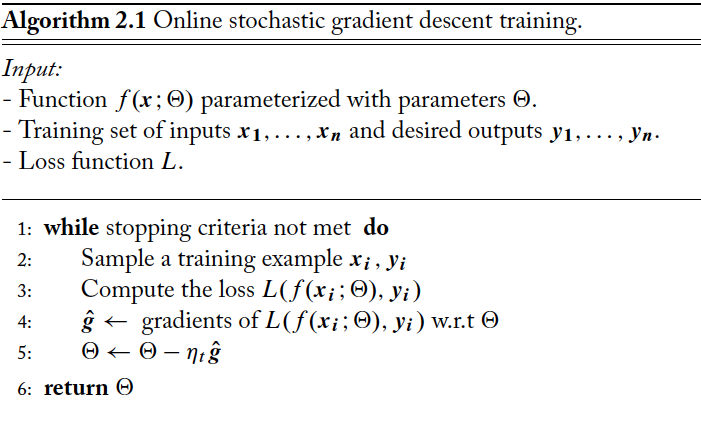
\includegraphics[scale=0.3]{pics/Online-SGD.png}
\end{figure}

\begin{scriptsize}
\begin{itemize}
\item The learning rate can either be fixed throughout the
training process, or decay as a function of the time step $t$.
\item  The error calculated in line 3 is based on a single training example, and is thus just a rough estimate of the corpus-wide loss $L$ that we are aiming to minimize. 
\item The noise in the loss computation may result in inaccurate gradients (single examples may provide noisy information).

\end{itemize}


\end{scriptsize}

\footnotetext{Source:\cite{goldberg2016primer}}

\end{frame}


\begin{frame}{Mini-batch Stochastic Gradient Descent}


\begin{scriptsize}
\begin{itemize}
\item A common way of reducing this noise is
to estimate the error and the gradients based on a sample of $m$ examples.
\item This gives rise to the minibatch SGD algorithm




\begin{figure}[htb]
	\centering
	 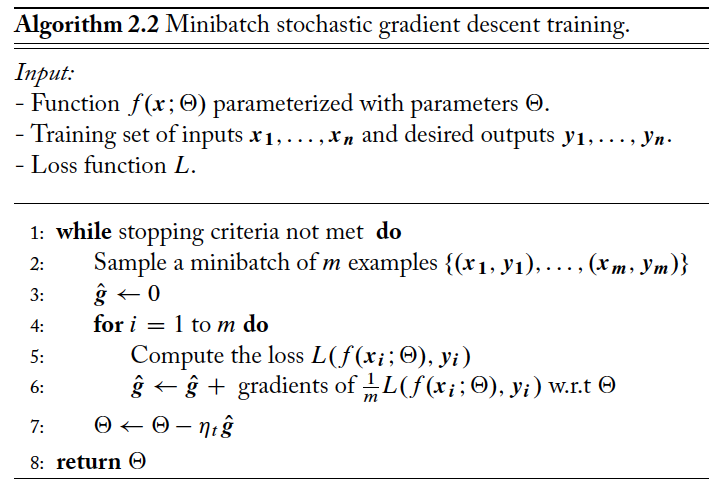
\includegraphics[scale=0.25]{pics/minibatch-SGD.png}
\end{figure}

\item Higher values of $m$ provide better estimates of the corpus-wide gradients, while smaller values allow more updates and in turn faster convergence.

\item For modest sizes of $m$ , some computing architectures (i.e., GPUs) allow an efficient parallel implementation of the computation in lines 3-6.

\end{itemize}
\end{scriptsize}

\footnotetext{Source:\cite{goldberg2016primer}}

\end{frame}



\begin{frame}{The Computation Graph Abstraction}
\begin{scriptsize}
\begin{itemize}
\item  One can compute the gradients of the various parameters of a network by hand and implement them in code.

\item This procedure is cumbersome and error prone.

\item For most purposes, it is preferable to use automatic tools for gradient computation [Bengio, 2012].

\item A computation graph is a representation of an arbitrary mathematical computation (e.g., a neural network) as a graph.

\item Consider for example a graph for the computation of $(a*b+1)*(a*b+2)$:

\begin{figure}[htb]
	\centering
	 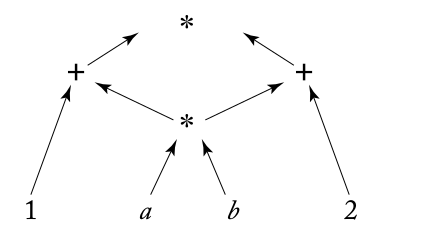
\includegraphics[scale=0.25]{pics/compGraph.png}
\end{figure}

\item The computation of $a*b$ is shared.

\item The graph structure defines the order of the computation in terms of the dependencies between the different components.

\end{itemize}
\end{scriptsize}
\end{frame}






\begin{frame}{The Computation Graph Abstraction}
\begin{scriptsize}
\begin{itemize}

\item  Te computation graph abstraction allows us to:


\begin{enumerate}
\begin{scriptsize}
 \item Easily construct arbitrary networks.
 \item Evaluate their predictions for given inputs (forward pass)
 
 \begin{figure}[htb]
	\centering
	 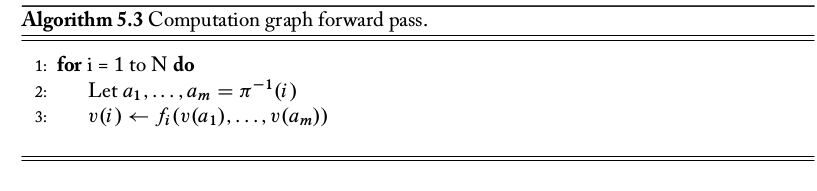
\includegraphics[scale=0.25]{pics/forwardPass.png}
\end{figure}

 
 
 \item Compute gradients for their parameters with respect to arbitrary scalar losses (backward pass or backpropagation).
 
 
  
 \begin{figure}[htb]
	\centering
	 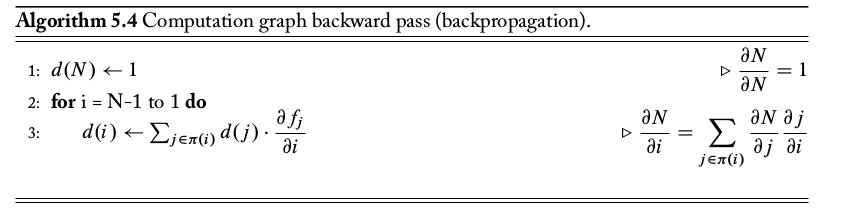
\includegraphics[scale=0.25]{pics/backwardPass.png}
\end{figure}
 
\end{scriptsize}
 \end{enumerate}
  
  
  
  
 \item The backpropagation algorithm (backward pass) is essentially following the chain-rule of differentiation\footnote{A comprehensive tutorial on the backpropagation algorithm over the computational graph abstraction: \url{https://colah.github.io/posts/2015-08-Backprop/}}.
 
 
 \item End of detour!
 
\end{itemize}
\end{scriptsize}
\end{frame}




\begin{frame}{Word2Vec}
\begin{scriptsize}
\begin{itemize}
\item Word2Vec is a software package that implements two neural network architectures for training word embeddings:  Continuos Bag of Words (CBOW) and Skip-gram.
\item It implements two  optimization models: Negative Sampling and Hierarchical Softmax.
\item These models are neural networks with one hidden layer that are trained to predict the contexts of words.
\end{itemize}
\end{scriptsize}
\end{frame}


% Good Word2Vec tutorial
%http://mccormickml.com/2016/04/19/word2vec-tutorial-the-skip-gram-model/

\begin{frame}{Skip-gram Model}
\begin{scriptsize}
\begin{itemize}
\item A neural network with one hidden layer is trained for predicting the words surrounding a center word, within a window  of size $k$ that is shifted along the input corpus. 
\item The center and surrounding $k$ words correspond to the input and output layers of the network.
\item Words are initially represented by 1-hot vectors: vectors of the size of the vocabulary ($|V|$) with zero values in all entries except for the corresponding word index that receives a value of 1. 
\item The output layer is formed by the concatenation of the $k$ 1-hot vectors of the surrounding words. 
\item The hidden layer has a dimensionality $d$, which determines the size of the embeddings (normally $d \ll |V|$).
\end{itemize}
\end{scriptsize}
  \begin{figure}[h]
        	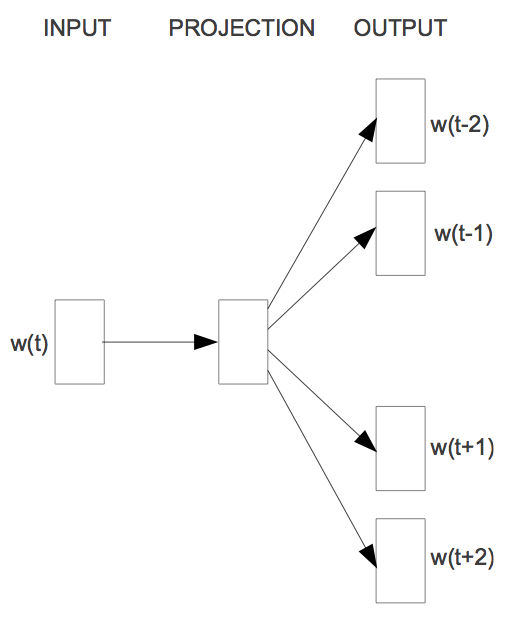
\includegraphics[scale = 0.33]{pics/skip-gram.png}
        \end{figure}

\end{frame}


\begin{frame}{Skip-gram Model}

  \begin{figure}[h]
        	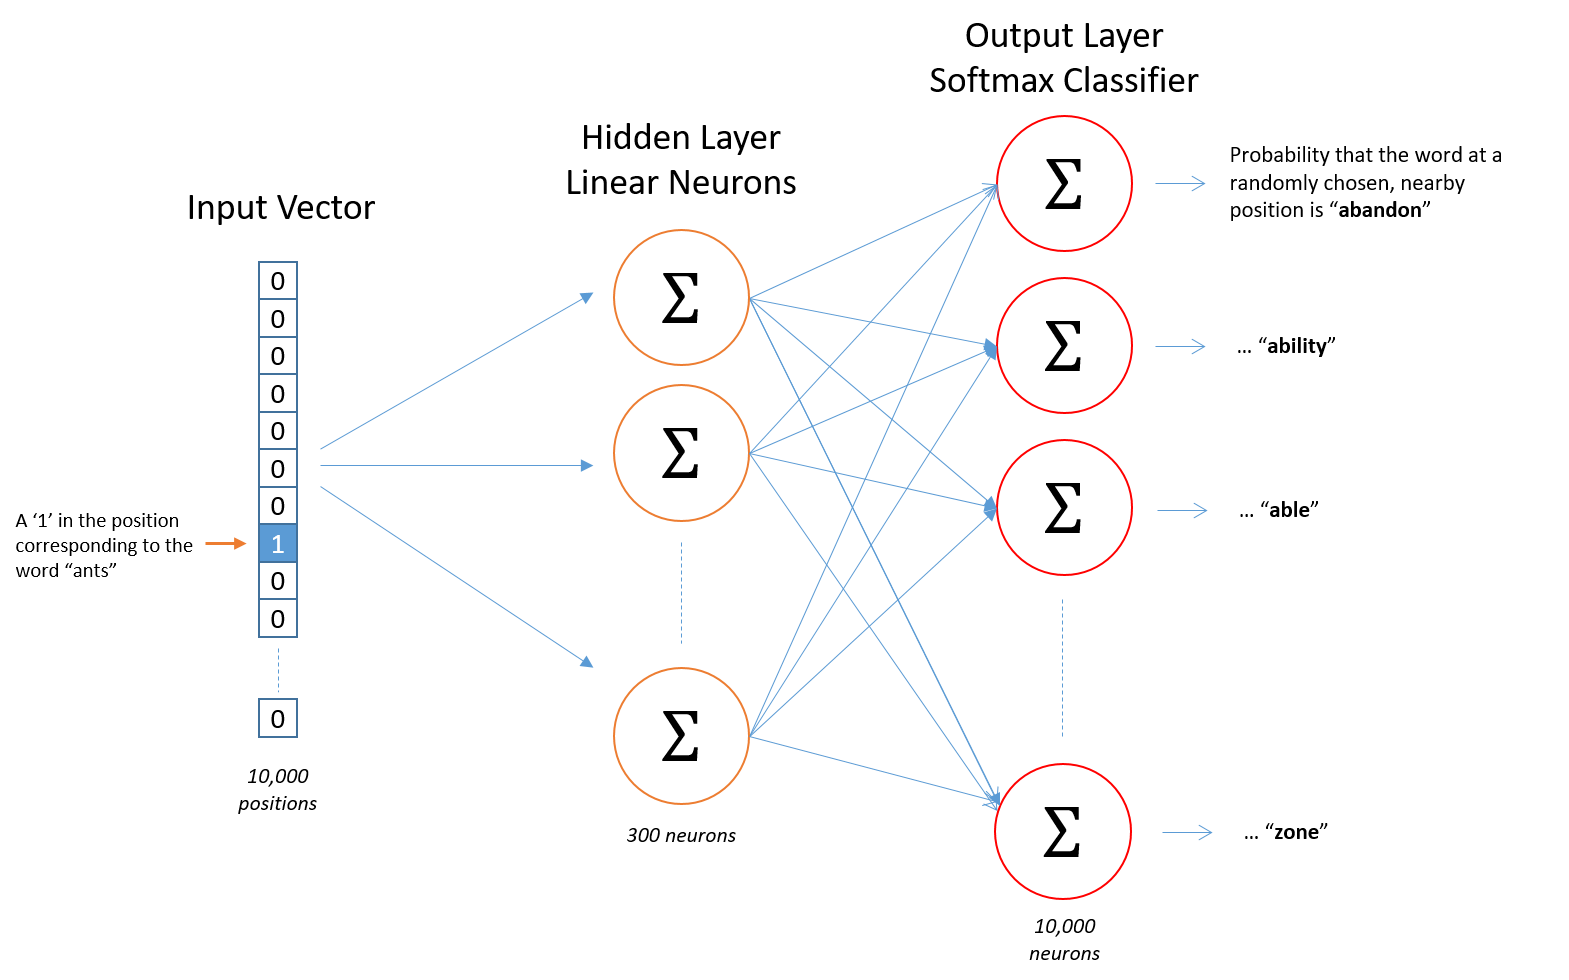
\includegraphics[scale = 0.4]{pics/skip_gram_net_arch.png}
        \end{figure}
\footnotetext{Picture taken from:    \url{http://mccormickml.com/2016/04/19/word2vec-tutorial-the-skip-gram-model/}}

\end{frame}


% we use hierarchical softmax where the vocabulary is represented as a Huffman binary tree. This follows previous observations that the frequency of words works well for obtaining classes in neural net language models [16]. Huffman trees assign short binary codes to frequent words, and this further reduces the number of output units that need to be evaluated


%If two different words have very similar “contexts” (that is, what words are likely to appear around them), then our model needs to output very similar results for these two words. And one way for the network to output similar context predictions for these two words is if the word vectors are similar. So, if two words have similar contexts, then our network is motivated to learn similar word vectors for these two words! Ta da!

%And what does it mean for two words to have similar contexts? I think you could expect that synonyms like “intelligent” and “smart” would have very similar contexts. Or that words that are related, like “engine” and “transmission”, would probably have similar contexts as well.

%This can also handle stemming for you – the network will likely learn similar word vectors for the words “ant” and “ants” because these should have similar contexts.

%https://arxiv.org/pdf/1402.3722.pdf

\begin{frame}{Parametrization of the Skip-gram model}
\begin{scriptsize}
\begin{itemize}
\item The conditional probability of the context word $c$ given the center word $w$ is modelled with a softmax ($C$ is the set of all context words):


\begin{displaymath}
p(c|w) = \frac{e^{\vec{c}\cdot \vec{w}}}{ \sum_{c'\in C} e^{\vec{c}'\cdot \vec{w}}}
\end{displaymath}



\item Model's parameters $\theta$: $\vec{c}$ and $\vec{w}$ (vector representations of contexts and words).
\item The optimization goal is to maximize the conditional likelihood of the contexts $c$:


\begin{equation}
\begin{split}
arg \max_{\vec{c}, \vec{w}} & \quad \sum_{(w,c) \in D}{\log p(c|w)} = \sum_{(w,c) \in D} ( \log e^{\vec{c}\cdot \vec{w}} - \log \sum_{c'\in C} e^{\vec{c}'\cdot \vec{w}}  )
\end{split}
\end{equation}


\item Assumption: maximising this function will result in good embeddings $\vec{w}$ i.e.,  similar words will have similar vectors.

\item The term $p(c|w)$ is computationally expensive because of the summation $\sum_{c'\in C} e^{\vec{c}'\cdot \vec{w}}$ over all the contexts $c'$

\item Fix: replace the softmax with a hierarchical softmax (the vocabulary is represented with a Huffman binary tree). 

\item Huffman trees assign short binary codes to frequent words, reducing the number of output units to be evaluated.

\end{itemize}
\end{scriptsize}
\end{frame}



%The distributional hypothesis states that words in similar contexts have similar meanings. The objective above clearly tries to increase the quantity  for good word-context pairs, and decrease it for bad ones.  Intuitively, this means that words that share many contexts will be similar to each other (notealso that contexts sharing many words will also be similar to each other). This is, however, very hand-wavy.

% https://arxiv.org/pdf/1402.3722.pdf  Skip-gram and Negative Sampling are not the same

\begin{frame}{Skip-gram with Negative Sampling}
\begin{scriptsize}
\begin{itemize}

\item Negative-sampling (NS) is presented as a more efficient model for calculating skip-gram embeddings. 
\item However, it optimises a different objective function \cite{goldberg2014word2vec}.

\item Let $D$ be the set of correct word-context pairs.

\item NS maximizes the probability that a word-context  pair a word-context pair $(w, c)$ came from the input corpus $D$ using a sigmoid function:

\begin{displaymath}
P(D = 1| w,c_i) = \frac{1}{1+e^{-\vec{w} \cdot \vec{c_{i}}}}
\end{displaymath}

\item Assumption: the contexts words $c_i$ are indepedent from each other:

\begin{displaymath}
P(D = 1| w,c_{1:k}) = \prod_{i=1}^{k}{P(D = 1| w,c_i)} = \prod_{i=1}^{k}{\frac{1}{1+e^{-\vec{w} \cdot \vec{c_{i}}}}} 
\end{displaymath}

\item This leads to the following target function (log-likelihood): 

\begin{equation}
\begin{split}
arg \max_{\vec{c}, \vec{w}} & \quad \log P(D = 1| w,c_{1:k}) = \sum_{i=1}^{k}{\log \frac{1}{1+e^{-\vec{w} \cdot \vec{c_{i}}}}}
\end{split}
\end{equation}





\end{itemize}
\end{scriptsize}
\end{frame}


\begin{frame}{Skip-gram with Negative Sampling (2)}
\begin{scriptsize}
\begin{itemize}


\item This objective has a trivial solution if we set $\vec{w}$,$\vec{c}$ such that $p(D=1|w,c)=1$ for every pair $(w,c)$ from $D$.
\item This is achieved by setting $\vec{w}=\vec{c}$  and $\vec{w} \cdot \vec{c} = K$ for all $\vec{w},\vec{c}$, where $K$ is a large number.
\item We need a mechanism that prevents all the vectors from having the same value, by disallowing some $(w, c)$ combinations. 
\item One way to do so, is to present the model with some $(w, c)$ pairs for which $p(D= 1|w, c)$ must be low, i.e.
pairs which are not in the data.  
\item This is achieved sampling negative samples from $\tilde{D}$. 





\end{itemize}
\end{scriptsize}
\end{frame}


\begin{frame}{Skip-gram with Negative Sampling (3)}
\begin{scriptsize}
\begin{itemize}

\item Sample $m$ words for each word-context pair  $(w,c) \in D$.
\item Add each sampled word $w_i$ together with the original context $c$ as a negative example to $\tilde{D}$.

%\item $\tilde{D}$ being $m$ times larger than $D$. 

%\item The number of negative samples $m$ is a parameter of the algorithm.

\item Final objective function:
\begin{equation}
\begin{split}
arg \max_{\vec{c}, \vec{w}} & \quad \sum_{(w,c) \in D}{\log P(D = 1| w,c_{1:k})} + \sum_{(w,c) \in \tilde{D}} \log P(D = 0| w,c_{1:k})
\end{split}
\end{equation}

\item The negative words are sampled from smoothed version of the corpus frequencies:
\begin{displaymath}
\frac{\#(w)^{0.75}}{\sum_{w'}\#(w')^{0.75}}
\end{displaymath}

\item This gives more relative weight to less frequent words.

\end{itemize}
\end{scriptsize}
\end{frame}






\begin{frame}{Continuos Bag of Words: CBOW}
\begin{scriptsize}
\begin{itemize}
\item  Similar to the skip-gram model but now the center word is predicted from the surrounding context.
 \begin{figure}[h]
    	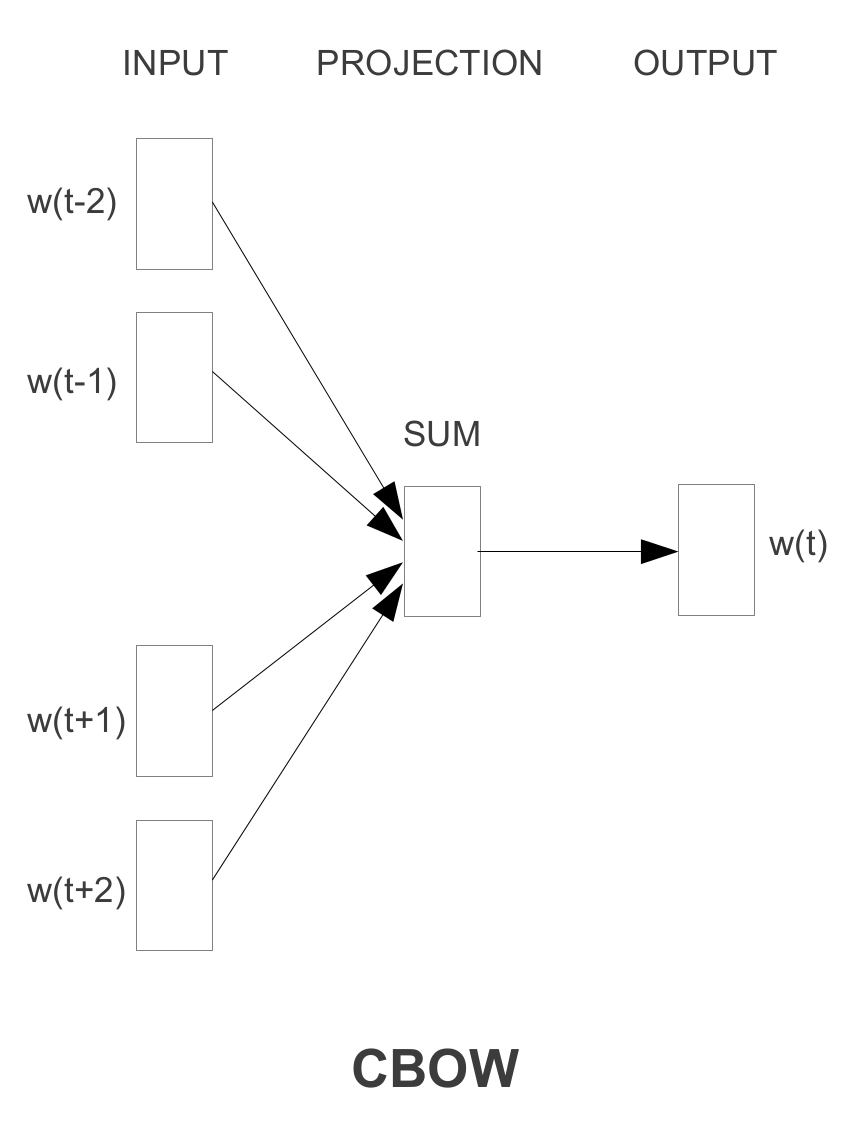
\includegraphics[scale = 0.55]{pics/CBOW.png}
    \end{figure}
       
        
\end{itemize}
\end{scriptsize}
\end{frame}



\begin{frame}{GloVe}
\begin{scriptsize}
\begin{itemize}
\item  GloVe (from global vectors) is another popular method for training word embeddings \cite{penningtonSM14}.

\item It constructs an explicit word-context
matrix, and trains the word and context vectors $\vec{w}$ and $\vec{c}$ attempting to satisfy:

\begin{equation}
w \cdot c + b_{[w]}+b_{[c]} = \log \#(w,c) \quad \forall (w,c) \in D
\end{equation}

\item where $b_{[w]}$ and $b_{[c]}$ are word-specific and context-specific trained biases.

        
\end{itemize}
\end{scriptsize}
\end{frame}



\begin{frame}{GloVe (2)}
\begin{scriptsize}
\begin{itemize}

\item In terms of matrix factorization, if we fix $b_{[w]}=\log \#(w)$ and $b_{[c]}=\log \#(c)$ we'll get an objective that is very similar to factorizing the word-context PMI matrix, shifted by $\log (|D|)$.
\item In GloVe the bias parameters are learned and not fixed, giving it another degree of freedom.

\item The optimization objective is weighted least-squares loss, assigning more weight to the correct reconstruction of frequent items.
       
\item When using the same word and context vocabularies, the model suggests representing each word as the sum of its corresponding word and context embedding vectors.   
        
\end{itemize}
\end{scriptsize}
\end{frame}


\begin{frame}{Word Analogies}
\begin{scriptsize}
\begin{itemize}
   
\item Word embeddings can capture certain semantic relationships, e.g. male-female, verb tense and country-capital relationships between words.

\item For example, the following relationship is found for word embeddings
trained using Word2Vec: $\vec{w}_{king} - \vec{w}_{man} + \vec{w}_{woman} \approx \vec{w}_{queen}$.

    
\end{itemize}

 \begin{figure}[h]
    	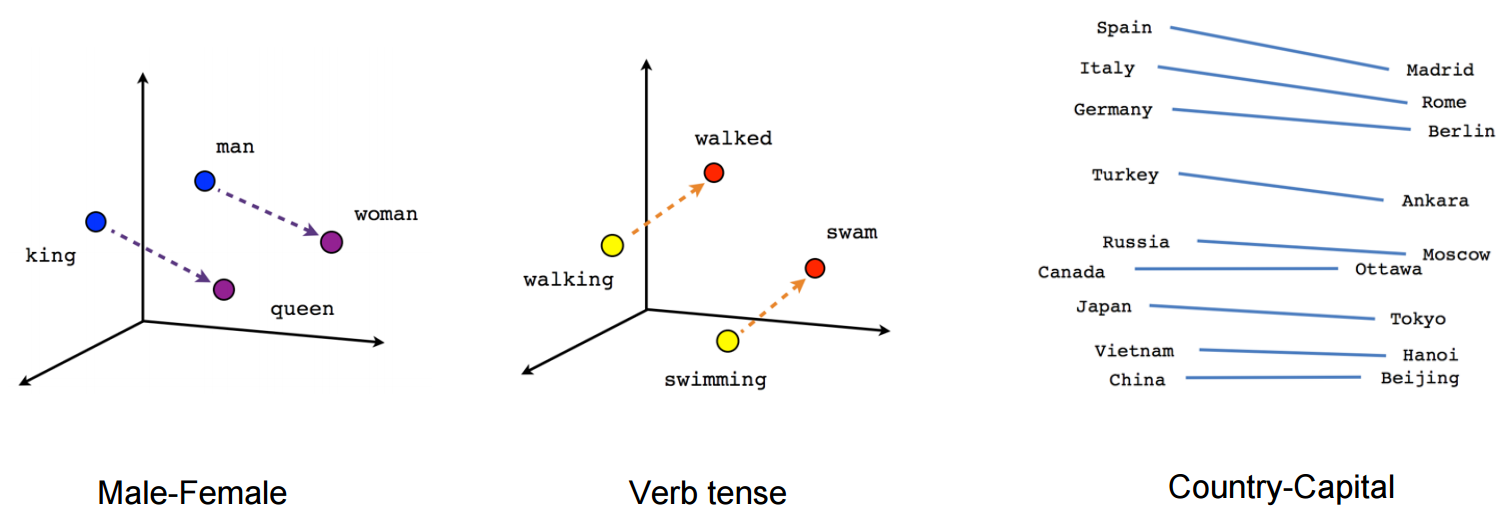
\includegraphics[scale = 0.2]{pics/linear-relationships.png}
    \end{figure}
\footnotemark{Source: \url{https://www.tensorflow.org/tutorials/word2vec}}

\end{scriptsize}
\end{frame}



\begin{frame}{Correspondence between Distributed and Distributional Models}
\begin{scriptsize}
\begin{itemize}
       
\item Both the distributional ``count-based'' methods and the distributed ``neural'' ones are based on the distributional hypothesis.

\item The both attempt to capture the similarity between words based on the similarity between the contexts in which they occur.      
       
\item Levy and Goldebrg showed in \cite{levy2014neural} that Skip-gram negative sampling (SGNS) is implicitly factorizing a word-context matrix, whose cells are the pointwise mutual information (PMI) of the respective word and context pairs, shifted by a global constant. 

%https://levyomer.files.wordpress.com/2014/09/neural-word-embeddings-as-implicit-matrix-factorization.pdf

\item This ties the neural methods and the traditional ``count-based'' suggesting that in a deep sense
the two algorithmic families are equivalent.
     
\end{itemize}
\end{scriptsize}
\end{frame}

\begin{frame}{Sentiment-Specific Phrase Embeddings}
%https://pdfs.semanticscholar.org/107f/b80ff801894b6191d0613af41aba91c134a4.pdf
\begin{scriptsize}
\begin{itemize}
\item Problem of word embeddings: antonyms can be used in similar contexts e.g., my car is nice vs my car is ugly.

\item In \cite{TangCol14}  \textbf{sentiment-specific} word embeddings are proposed  by combining the skip-gram model with emoticon-annotated tweets :) :( .

\item These embeddings are used for \textbf{training} a word-level polarity classifier.

\item The model integrates sentiment information into the continuous representation of phrases by developing a tailored neural architecture.

\item Input: $\{w_i,s_j,pol_j\}$, where $w_i$ is a phrase (or word), $s_j$ the sentence, and $pol_j$ the sentece's polarity.

\end{itemize}
\end{scriptsize}
\end{frame}


\begin{frame}{Sentiment-Specific Phrase Embeddings (2)}
%https://pdfs.semanticscholar.org/107f/b80ff801894b6191d0613af41aba91c134a4.pdf
\begin{scriptsize}
\begin{itemize}

\item The training objective uses the embedding of $w_i$ to predict its context words (in the same way as the skip-gram model), and uses the sentence representation $se_j$ to predict $pol_j$.


\item Sentences ($se_j$) are represented by averaging the word vectors of their words.

\item The  objective of the sentiment part is to maximize the average of log sentiment probability: 
\begin{displaymath}
f_{sentiment}= \frac{1}{S}\sum_{j=1}^{S}\log p(pol_j|se_j)
\end{displaymath}

\item The final training objective is to maximize the linear combination of the skip-gram and sentiment objectives: 
\begin{displaymath}
f = \alpha f_{skipgram} + (1- \alpha)f_{sentiment}
\end{displaymath}

\end{itemize}
\end{scriptsize}
\end{frame}



\begin{frame}{Sentiment-Specific Phrase Embeddings}
%https://pdfs.semanticscholar.org/107f/b80ff801894b6191d0613af41aba91c134a4.pdf


  \begin{figure}[h]
        	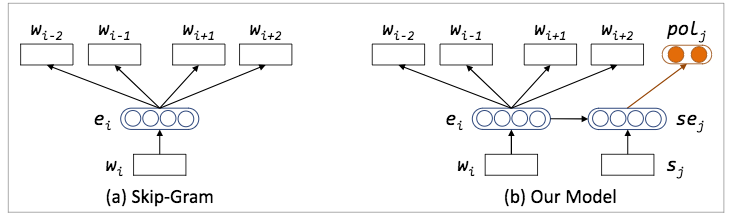
\includegraphics[scale = 0.4]{pics/SSPE.png}
        \end{figure}

  \begin{figure}[h]
        	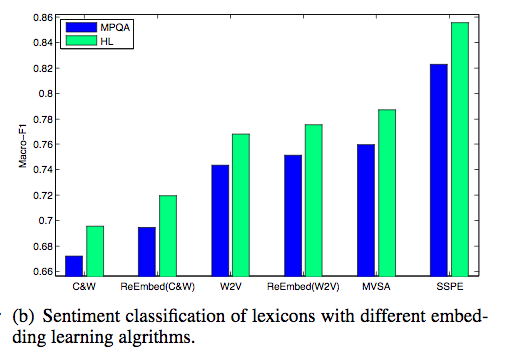
\includegraphics[scale = 0.3]{pics/SSPERes.png}
        \end{figure}


\end{frame}






\begin{frame}{Multi-Label Classification of Emotions with TCM}
\begin{scriptsize}

\begin{figure}[htbp]
\begin{center}
\scalebox{0.7}{
\begin{tabular}{cccc}
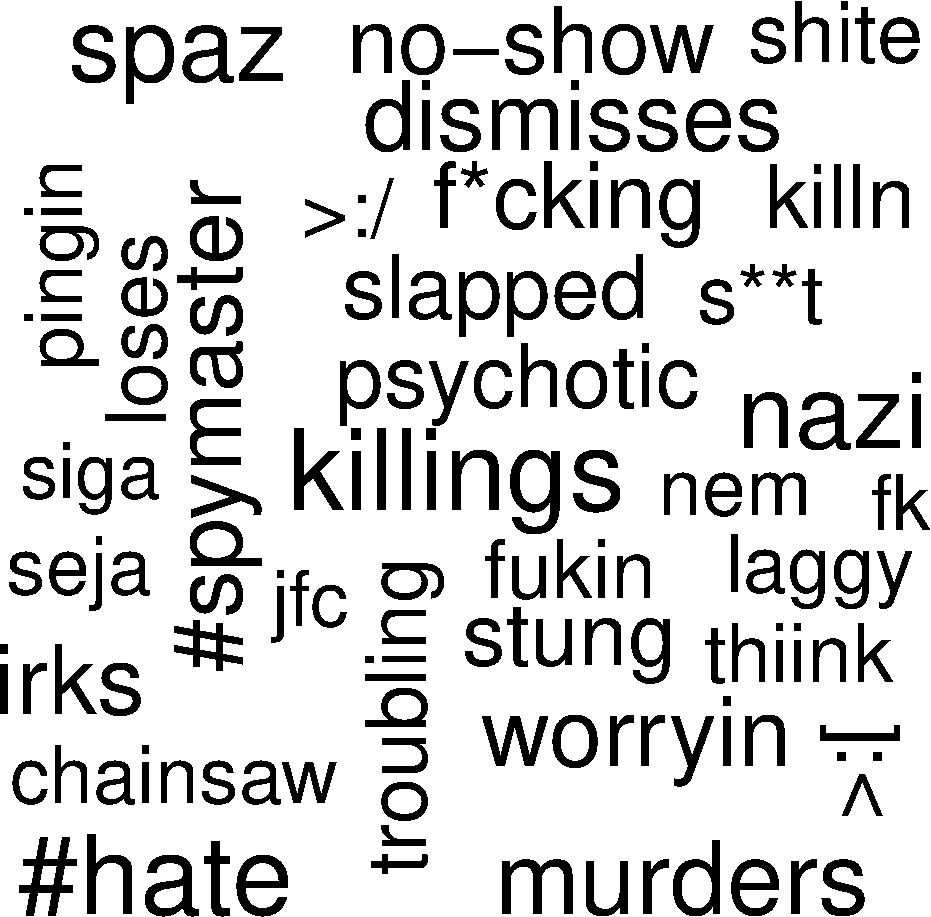
\includegraphics[scale=0.2]{pics/anger.pdf} & 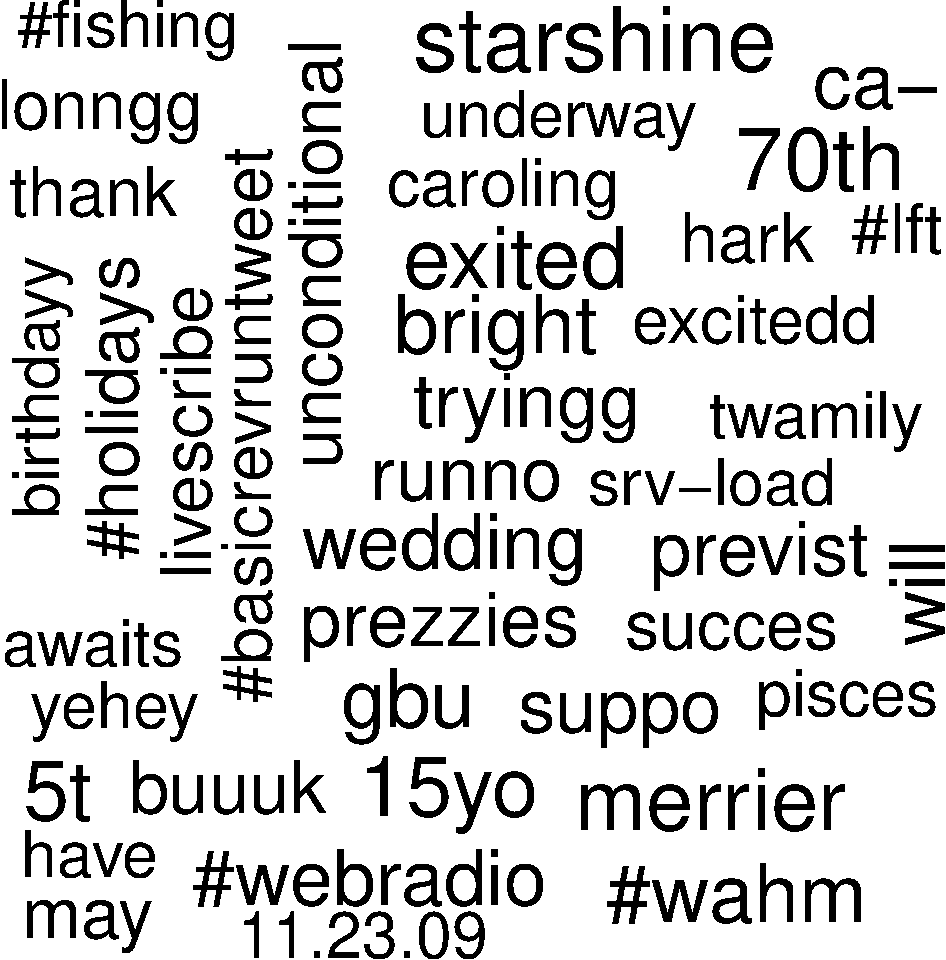
\includegraphics[scale=0.2]{pics/ant.pdf} & 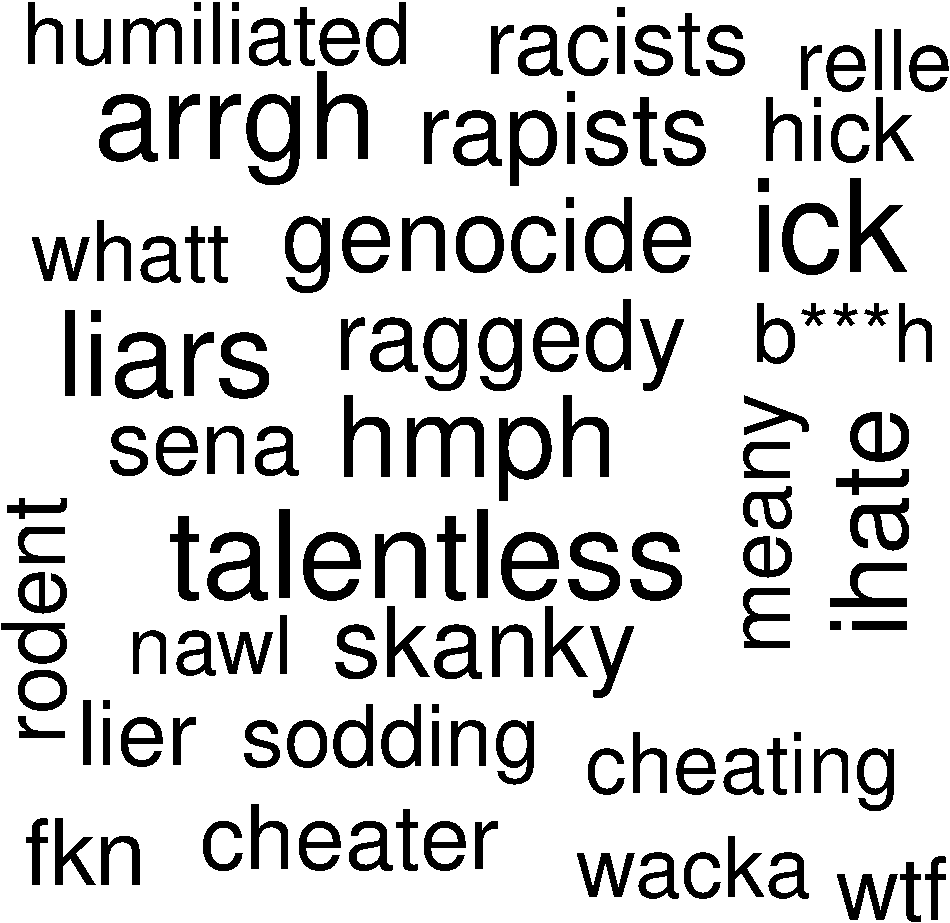
\includegraphics[scale=0.2]{pics/disg.pdf} & 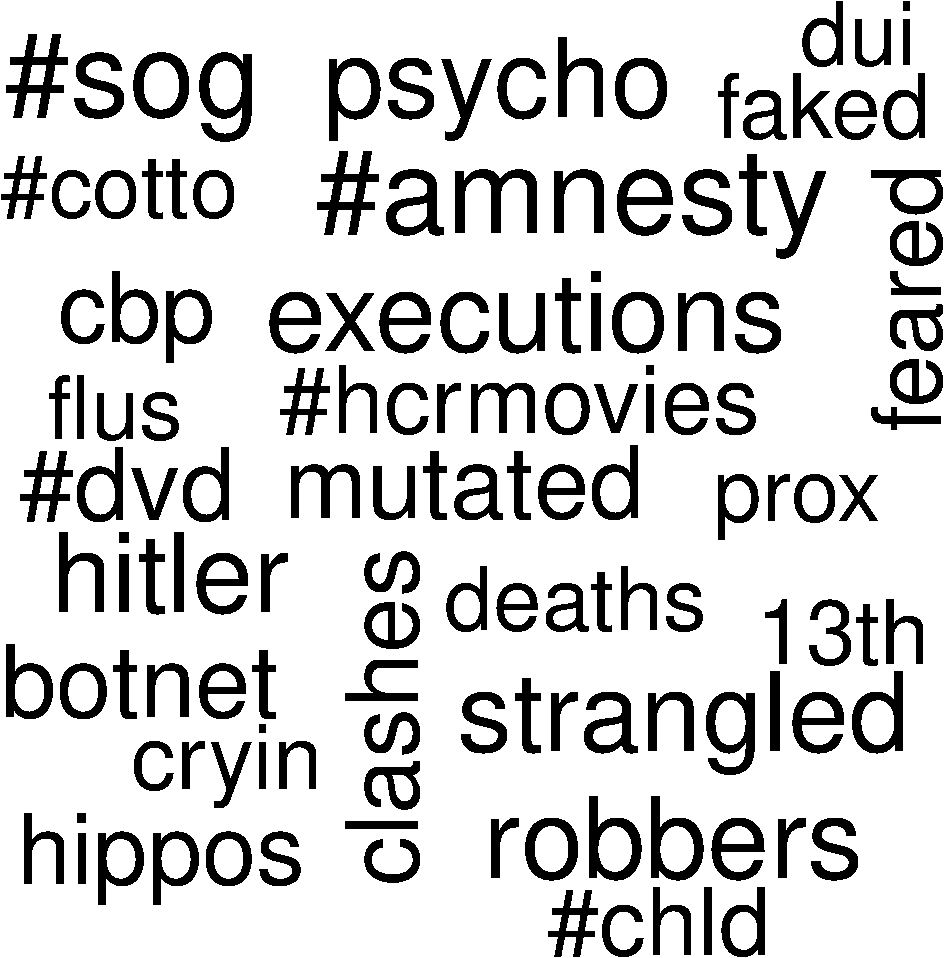
\includegraphics[scale=0.2]{pics/fear.pdf} \\
anger & anticipation & disgust & fear\\[1mm] 
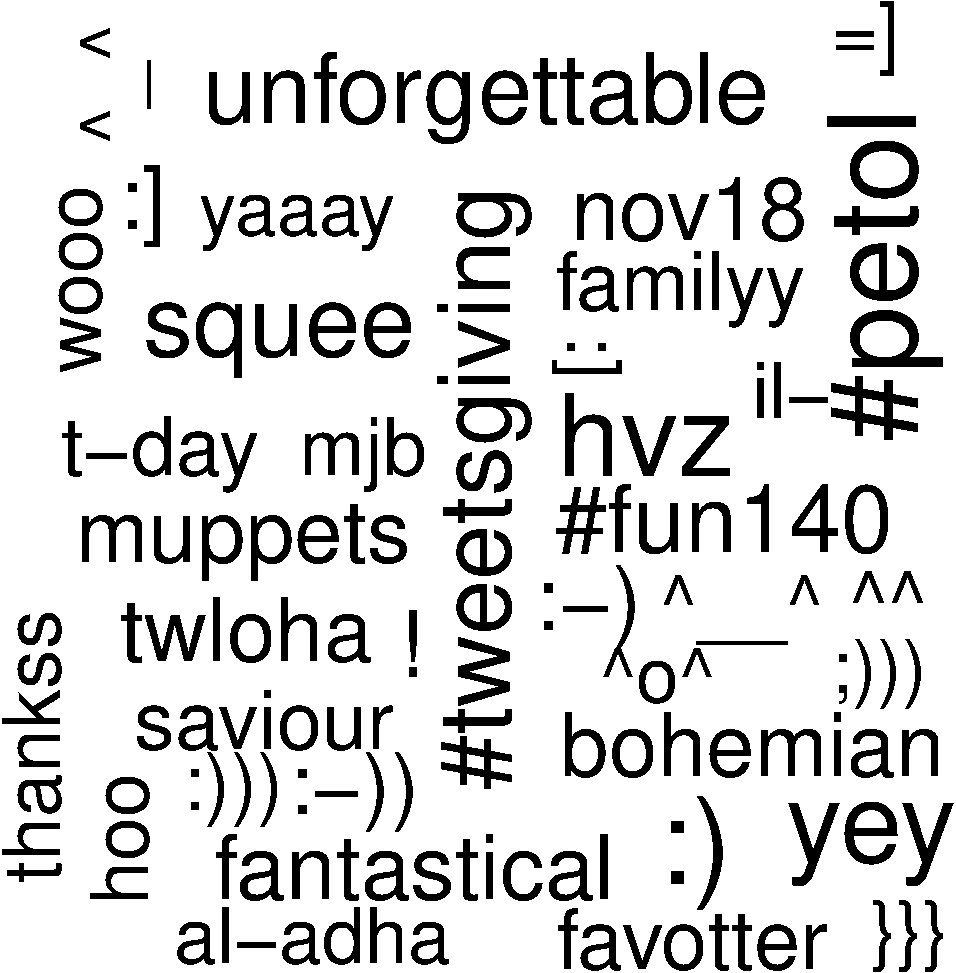
\includegraphics[scale=0.2]{pics/joy.pdf} & 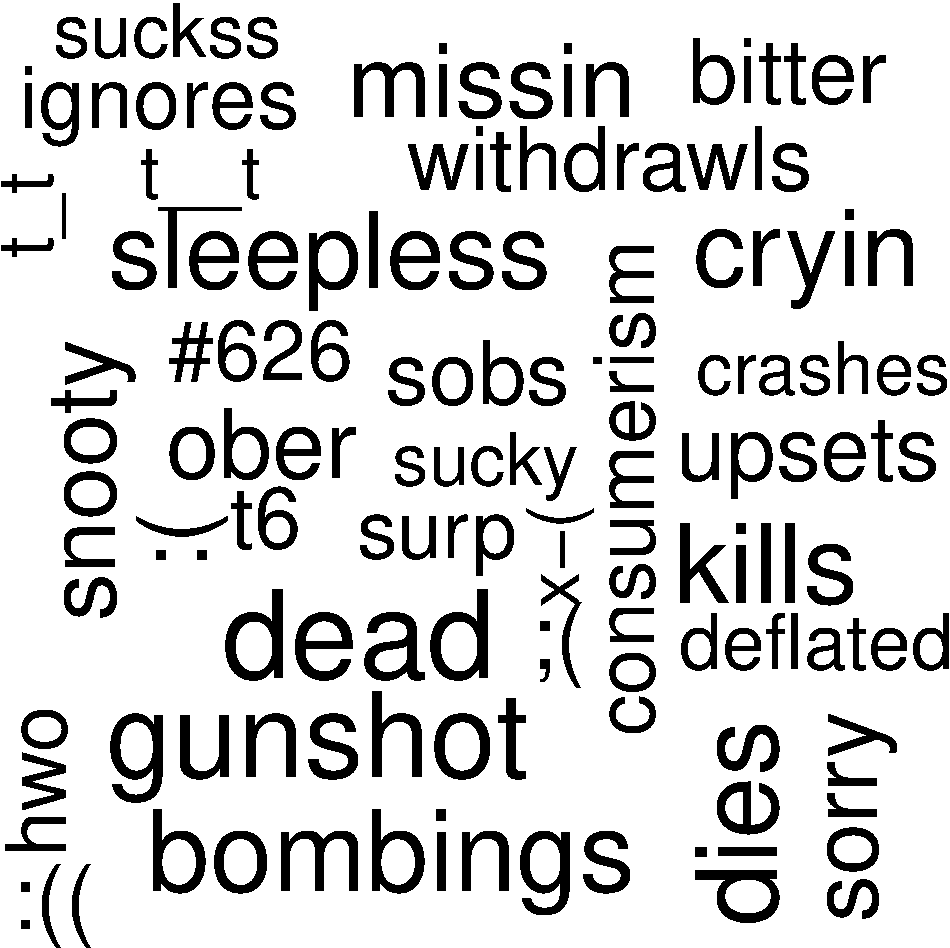
\includegraphics[scale=0.2]{pics/sadness.pdf} & 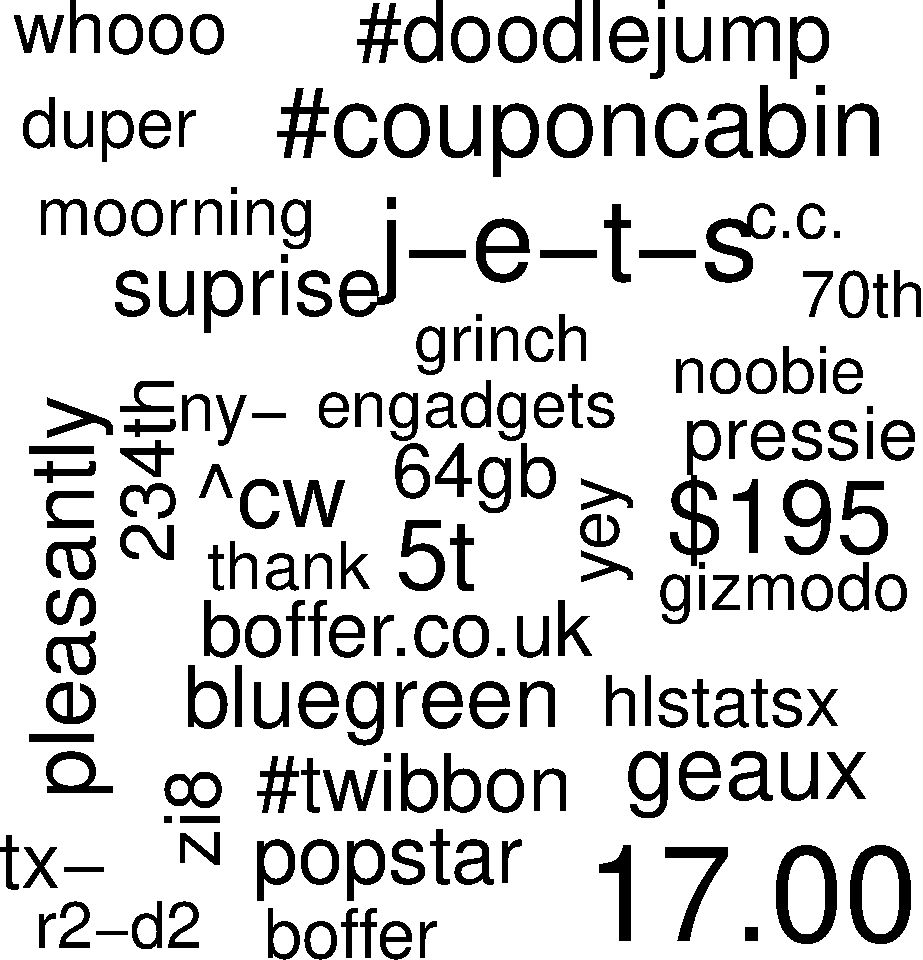
\includegraphics[scale=0.2]{pics/surprise.pdf} & 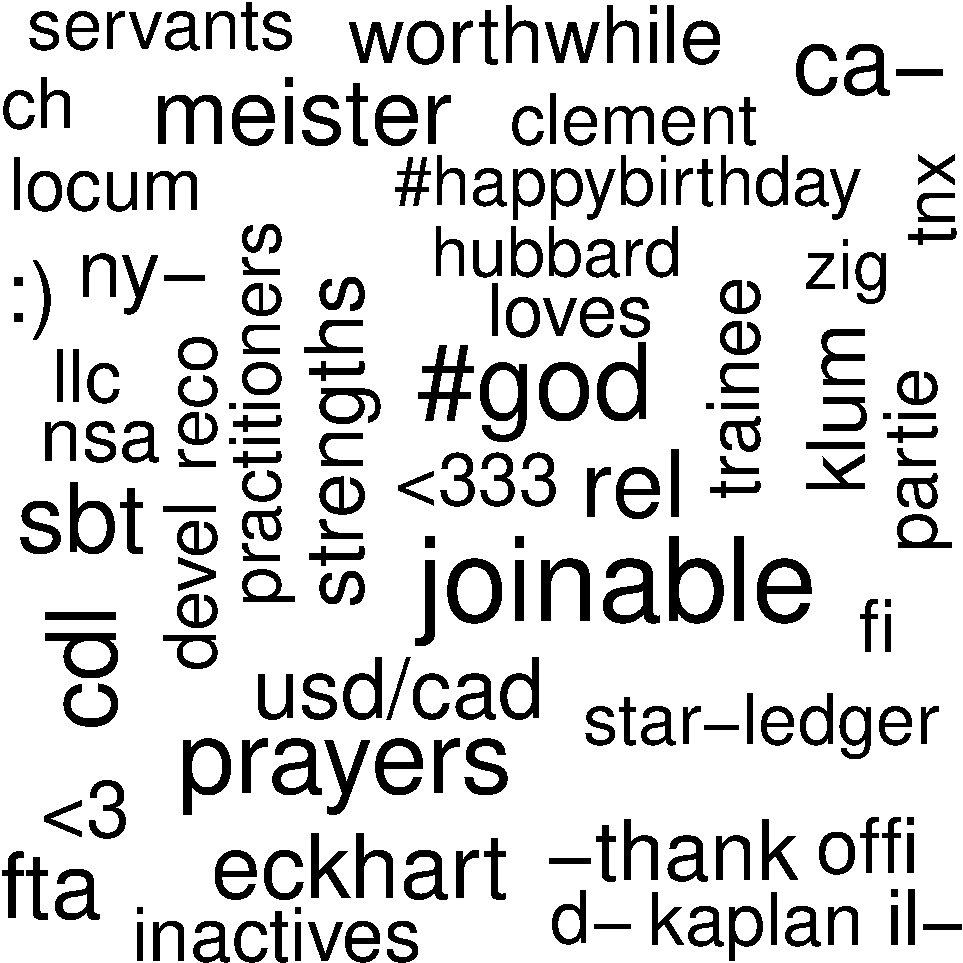
\includegraphics[scale=0.2]{pics/trust.pdf} \\
joy & sadness & surprise & trust\\
\end{tabular}}
\end{center}
\end{figure}

\end{scriptsize}
\end{frame}



\section{Message-level Sentiment Classification}




\begin{frame}{Convolutional Neural Networks}
\begin{scriptsize}
\begin{itemize}
\item Convolutional neural networks (CNNs) became very popular in the computer vision community due to its success for detecting objects (``cat'',``bicycles'') regardless of its position in the image.
\item They identify indicative local predictors in a structure (e.g., images, sentences).
\item These predictors are combined to produce a fixed size vector representation for the structure.
\item When used in NLP, the network captures the n-grams that are most informative for the target predictive task.
\item For sentiment classification, these local aspects correspond to n-grams conveying sentiment (e.g., not bad, very good).
\item The fundamental idea of CNNs \cite{lecun1998gradient}  is  to  consider  feature extraction and classification as one jointly trained task. 

\end{itemize}
\end{scriptsize}
\end{frame}

\begin{frame}{Basic Convolution  + Pooling}
\begin{scriptsize}
\begin{itemize}
\item Sentences are usually modelled as sequences of word embeddings.
\item The CNN applies  nonlinear (learned) functions or ``filters'' mapping windows of $k$ words into scalar values.
\item Several filters can be applied, resulting in an $l$-dimensional vector (one dimension per filter).
\item The filters capture relevant properties of the words in the window.
\item These filters correspond to the ``convolution layer'' of the network.
\end{itemize}
\end{scriptsize}
\end{frame}

\begin{frame}{Basic Convolution  + Pooling}
\begin{scriptsize}
\begin{itemize}
\item The ``pooling'' layer is used
to combine the vectors resulting from the different windows into a single $l$-dimensional vector.
\item This is done by taking the max or the average value observed in each of the dimensions over the different windows.
\item The goal is to capture the most important ``features'' in the sentence, regardless of the position.
\item The resulting $l$-dimensional vector is then fed further into a network that is used for prediction (e.g., softmax).
\item The gradients are propagated back from the network's loss tuning the parameters of the filter.
\item The filters learn to highlight the aspects of the data (n-grams) that are important for the target task. 
\end{itemize}
\end{scriptsize}
\end{frame}



\begin{frame}{Basic Convolution  + Pooling}
  \begin{figure}[h]
        	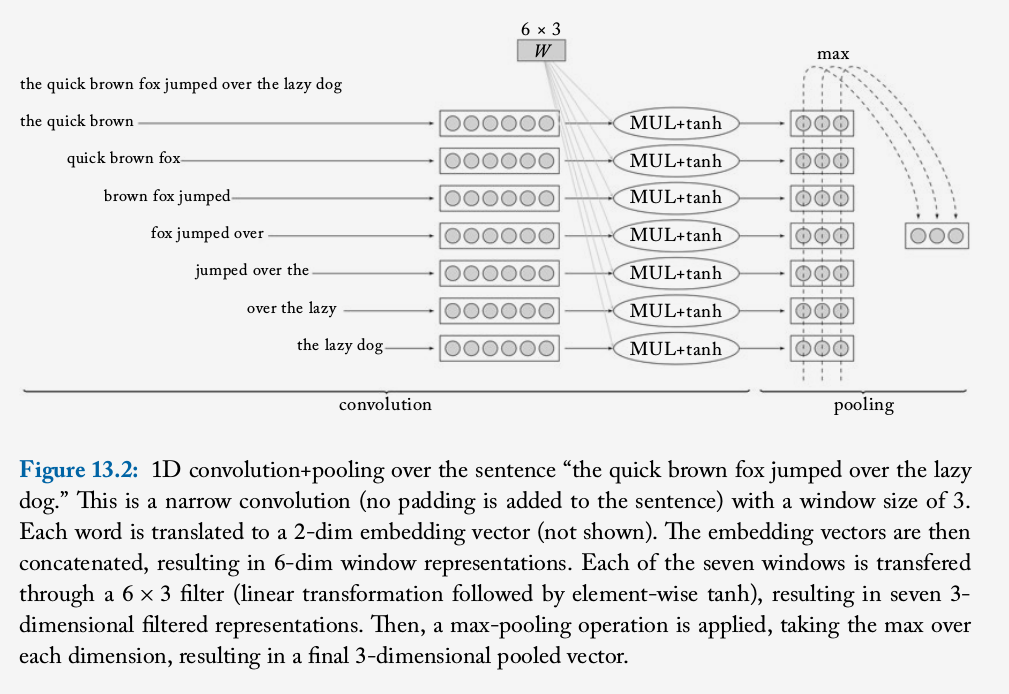
\includegraphics[scale = 0.28]{pics/CNN.png}
        \end{figure}
 \footnotemark{Source: \cite{goldberg2016primer}}   
\end{frame}



\begin{frame}{1D Convolutions over Text}
\begin{scriptsize}
\begin{itemize}
\item We focus on the one-dimensional convolution operation\footnote{1D here refers to a convolution operating over 1-dimensional inputs such as sequences, as opposed to 2D convolutions which
are applied to images.}.
\item Consider a sequence of words $w_{1:n}=w_1 ,\dots,w_n$ each with their corresponding $d_{emb}$ dimensional word embedding $E_{[w_i]}=\vec{w}_{i}$.
\item A 1D convolution of width $k$ works by moving a sliding-window of size $k$ over the sentence, and applying the same filter to each window
in the sequence.
\item A filter is a dot-product with a weight vector $\vec{u}$ , which is often followed by a nonlinear activation function.
\end{itemize}
\end{scriptsize}
\end{frame}

\begin{frame}{1D Convolutions over Text}
\begin{scriptsize}
\begin{itemize}
\item Define the operator $\oplus (w_{i:i+k-1})$ to be the concatenation of the vectors $\vec{w}_{i}, \dots, \vec{w}_{i+k-1}$.
\item The concatenated vector of the $i$-th window is $\vec{x}_{i}=\oplus (w_{i:i+k-1}) = [\vec{w}_{i};\vec{w}_{i+1};\dots;\vec{w}_{i+k-1}]$, $x_{i} \in \mathcal{R}^{k \cdot d_{emb}}$.
\item We then apply the filter to each window vector resulting in scalar values $p_{i} =  g(\vec{x}_{i} \cdot \vec{u})$. ($p_{i} \in \mathcal{R}$)
\item It is customary to use $l$ different filters, $\vec{u}_1,\dots, \vec{u}_l$, which can be arranged into a matrix $U$, and a bias vector $\vec{b}$ is often added: $\vec{p}_{i}=g(\vec{x}_{i}\cdot U +\vec{b})$.

\item Each vector $\vec{p}_i$ is a collection of $l$ values that represent (or summarise) the $i$-th window ($\vec{p}_{i} \in \mathcal{R}^l$). 
\item Ideally, each dimension captures a different kind of indicative information.

\end{itemize}
\end{scriptsize}
\end{frame}


\begin{frame}{Narrow vs. Wide Convolutions}
\begin{scriptsize}
\begin{itemize}
\item How many vectors $\vec{p}_i$ do we have?
\item For a sentence of length $n$ with a window of size $k$, there are $n - k + 1$ positions in which to start the sequence. 
\item We get $n - k + 1$ vectors $\vec{p}_{1:n-k+1}$. 
\item This approach is called \textbf{narrow convolution}.
\item An alternative is to pad the sentence with $k - 1$ padding-words to each side, resulting in $n+k+1$ vectors $\vec{p}_{1:n+k+1}$. 
\item This is called a \textbf{wide convolution}.
\end{itemize}
\end{scriptsize}
\end{frame}


\begin{frame}{1D Convolutions over Text}
\begin{scriptsize}
\begin{itemize}
\item The main idea behind the convolution layer is to apply the same parameterised function over all $k$-grams in the sequence.
\item This creates a sequence of $m$ vectors, each representing
a particular $k$-gram in the sequence.
\item The representation is sensitive to the identity and order of the words within a $k$-gram.
\item However, the same representation will be extracted for a $k$-gram regardless of its position within the sequence.
\end{itemize}
\end{scriptsize}
\end{frame}



\begin{frame}{Vector Pooling}
\begin{scriptsize}
\begin{itemize}
\item Applying the convolution over the text results in $m$ vectors $\vec{p}_{1:m}$, each $\vec{p}_i \in \mathcal{R}^l$.
\item These vectors are then combined (pooled) into a single vector $c \in \mathcal{R}^l$ representing the entire sequence.
\item Max pooling: this operator takes the maximum value across each dimension (most common pooling operation).
\begin{displaymath}
c_[j]= \max_{1< i \leq m} p_{i[j]} \quad \forall j \in [1,l]
\end{displaymath}

\item Average Pooling (second most common): takes the average value of each index:
\begin{displaymath}
c = \frac{1}{m} \sum_{i=1}^{m}p_i
\end{displaymath}

\item Ideally, the vector $c$ will capture the essence of the important information in the sequence. 

\end{itemize}
\end{scriptsize}
\end{frame}



\begin{frame}{Vector Pooling}
\begin{scriptsize}
\begin{itemize}
\item The nature of the important information that needs to be encoded in the vector $c$ is task dependent. 
\item If we are performing sentiment classification, the essence are informative ngrams that indicate
sentiment.
\item If we are performing topic-classification, the essence are informative $n$-grams that indicate a particular topic.

\item During training, the vector $c$ is fed into downstream network layers (i.e., an MLP), culminating in an output layer which is used for prediction.
\item The training procedure of the network calculates the loss with respect to the prediction task, and the error gradients are propagated all the way back through the pooling and convolution layers, as well as the embedding layers. 
\item The training process tunes the convolution matrix $U$, the bias vector $\vec{b}$, the downstream network, and
potentially also the embeddings matrix $E$\footnote{While some people leave the embedding layer fixed during training, others allow the parameters to change.}  such that the vector $c$ resulting from the convolution
and pooling process indeed encodes information relevant to the task at hand.
\end{itemize}
\end{scriptsize}
\end{frame}



\begin{frame}{Twitter Sentiment Classification with CNN}
\begin{scriptsize}
\begin{itemize}
\item A convolutional neural network architecture for Twitter sentiment classification is developed in \cite{Severyn2015}.
\item  Each tweet is represented as a matrix whose columns correspond to the words in the tweet, preserving the order in which they occur.
\item  The words are represented by dense vectors or embeddings trained from a large corpus of unlabelled tweets using word2vec.
\item  The network is formed by the following layers: an input layer with the given tweet matrix, a  single  convolutional layer, a rectified linear activation function, a max pooling layer, and a soft-max classification layer.
\end{itemize}
\end{scriptsize}
\end{frame}


\begin{frame}{Twitter Sentiment Classification with CNN}
\begin{scriptsize}
\begin{itemize}
\item  The weights of the neural network are pre-trained using emoticon-annotated data, and then trained with the hand-annotated tweets from the SemEval competition.
\item   Experimental results show that the pre-training phase allows for a proper initialisation of the network's weights, and hence, has a positive impact on classification accuracy. 
\end{itemize}
  \begin{figure}[h]
        	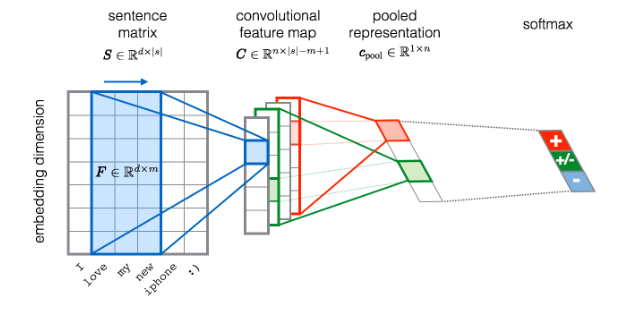
\includegraphics[scale = 0.45]{pics/cnn-twitter.png}
        \end{figure}
\end{scriptsize}
\end{frame}




\begin{frame}{Very Deep Convolutional Networks for Text Classification}
\begin{scriptsize}
\begin{itemize}
\item CNNs architectures for NLP are rather shallow in comparison to the deep convolutional networks which have pushed the state-of-the-art in computer vision.
\item A new architecture (VDCNN) for text processing which operates directly at the character level and uses only small convolutions and pooling operations is proposed in \cite{conneau2017very}.

\item Character-level embeddings are used instead of word-embeddings.

\item Characters are the lowest atomic representation of text. 

\item The performance of this model increases with depth: using up to 29 convolutional layers, authors report improvements over the state-of-the-art on several public text classification tasks. 

\item Most notorious improvements are achieved on large datasets.

\item First paper showing the the benefits  of  depth architectures for NLP.
\end{itemize}
\end{scriptsize}
\end{frame}






\begin{frame}{Very Deep Convolutional Networks for Text Classification}

  \begin{figure}[h]
        	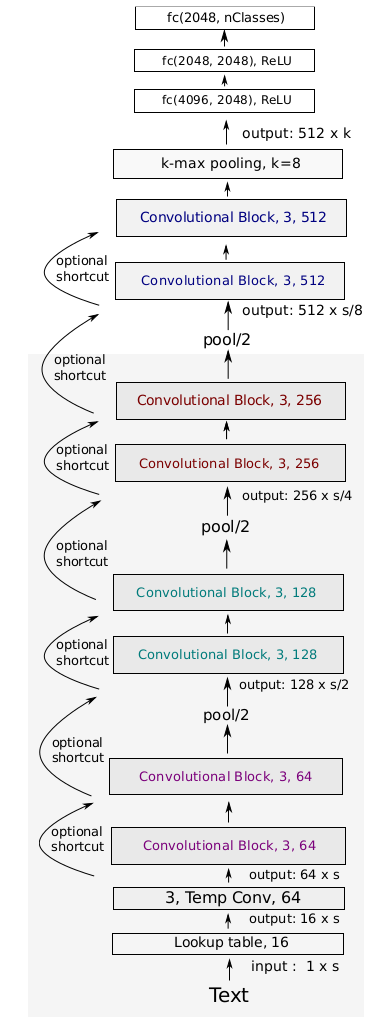
\includegraphics[scale = 0.2]{pics/VDCNN.png}
        \end{figure}

\end{frame}



\begin{frame}{Recurrent Neural Networks}
\begin{scriptsize}
\begin{itemize}

\item While representations derived from convolutional networks  offer some sensitivity to word order, their order sensitivity is restricted to mostly local patterns, and disregards the order of patterns that are far apart in the sequence.
\item Recurrent neural networks (RNNs) allow representing arbitrarily sized sequential inputs in fixed-size vectors, while paying attention to the structured properties of the inputs \cite{goldberg2016primer}.
\item RNNs, particularly ones with gated architectures such as the LSTM and the GRU, are very powerful at capturing statistical regularities in sequential inputs.

\end{itemize}
\end{scriptsize}
\end{frame}


\begin{frame}{The RNN Abstraction}
\begin{scriptsize}
\begin{itemize}

\item We use $\vec{x}_{i:j}$ to denote the sequence of vectors $\vec{x}_i, \dots, \vec{x}_j$.

\item On a high-level, the RNN is a function that takes as input an arbitrary length ordered sequence of $n$ $d_{in}$-dimensional vectors $\vec{x}_{i:n}=\vec{x}_1,\vec{x}_2, \dots, \vec{x}_n$ ( $\vec{x}_i \in  \mathcal{R}^{d_{in}}$) and returns as output a single $d_{out}$ dimensional vector $\vec{y}_n$ $\in \mathcal{R}^{d_{out}}$:

\begin{equation}
\begin{split}
\vec{y}_n & = RNN(\vec{x}_{1:n}) \\
\vec{x}_i \in  \mathcal{R}^{d_{in}} & \quad  \vec{y}_n  \in \mathcal{R}^{d_{out}}
\end{split}
\end{equation}

\item This implicitly defines an output vector $\vec{y}_i$ for each prefix $\vec{x}_{1:i}$ of the sequence $\vec{x}_{i:n}$.
\item We denote by $RNN^{*}$ the function returning this sequence:
\begin{equation}
\begin{split}
\vec{y}_{1:n} & = RNN^{*}(\vec{x}_{1:n}) \\
\vec{y}_i & = RNN(\vec{x}_{1:i}) \\
\vec{x}_i \in  \mathcal{R}^{d_{in}} & \quad  \vec{y}_n  \in \mathcal{R}^{d_{out}}
\end{split}
\end{equation}

\end{itemize}
\end{scriptsize}
\end{frame}


\begin{frame}{The RNN Abstraction}
\begin{scriptsize}
\begin{itemize}

\item The output vector $\vec{y}_n$ is then used for further prediction.
\item For example, a model for predicting the conditional probability of an event $e$ given the sequence $\vec{x}_{1:n}$ can be defined as the $j$-th element in the output vector resulting from the softmax operation over a linear transformation of the RNN encoding:
\begin{displaymath}
p(e = j|\vec{x}_{1:n}) = \text{softmax}(RNN(\vec{x}_{1:n})\cdot W +b)_{[j]} 
\end{displaymath}
\item The RNN function provides a framework for conditioning on the entire history without resorting to the Markov assumption which is traditionally used for modeling sequences.
\end{itemize}
\end{scriptsize}
\end{frame}



\begin{frame}{The RNN Abstraction}
\begin{scriptsize}
\begin{itemize}
\item The RNN is defined recursively, by means of a function $R$ taking as input a state vector $\vec{s}_{i-1}$  and an input vector $\vec{x}_{i}$ and returning a new state vector $\vec{s}_i$. 
\item The state vector $\vec{s}_i$ is then mapped to an output vector $\vec{y}_i$ using a simple deterministic function $O(\cdot)$.
\item The base of the recursion is an initial state vector, $\vec{s}_{0}$ , which is also an input to the RNN.
\item For brevity, we often omit the initial vector $s_{0}$ , or assume it is the zero vector.
\item When constructing an RNN, much like when constructing a feed-forward network, one has to specify the dimension of the inputs $\vec{x}_i$ as well as the dimensions of the outputs $\vec{y}_i$. 
\end{itemize}
\end{scriptsize}
\end{frame}




\begin{frame}{The RNN Abstraction}
\begin{scriptsize}

\begin{equation}
\begin{split}
 RNN^{*}(\vec{x}_{1:n};\vec{s}_0) & = \vec{y}_{1:n} \\
\vec{y}_i & = O(\vec{s}_i) \\
\vec{s}_i & = R(\vec{s}_{i-1},\vec{x}_i) \\
\vec{x}_i \in \mathcal{R}^{d_{in}}, & \quad \vec{y}_i \in \mathcal{R}^{d_{out}}, \quad \vec{s}_i \in \mathcal{R}^{f(d_{out})}
\end{split}
\end{equation}
\begin{itemize}
\item The functions $R$ and $O$ are the same across the sequence positions. 
\item The RNN keeps track of the states of computation through the state vector $\vec{s}_i$ that is kept and being passed across invocations of $R$.


\end{itemize}
\end{scriptsize}
\end{frame}




\begin{frame}{The RNN Abstraction}
\begin{scriptsize}

  \begin{figure}[h]
        	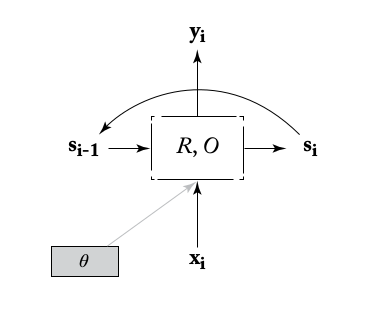
\includegraphics[scale = 0.4]{pics/RNN.png}
        \end{figure}
\begin{itemize}
\item This presentation follows the recursive definition, and is correct for arbitrarily long sequences.
\end{itemize}
\end{scriptsize}
\end{frame}




\begin{frame}{The RNN Abstraction}
\begin{scriptsize}
\begin{itemize}
\item For a finite sized input sequence (and all input sequences we deal with are finite) one can unroll the recursion.
  \begin{figure}[h]
        	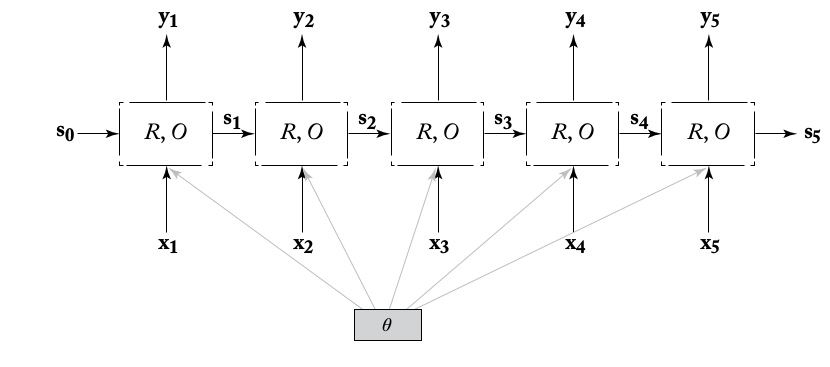
\includegraphics[scale = 0.35]{pics/RNN-unrolled.png}
        \end{figure}

        
\item The parameters $\theta$ highlight the fact that the same parameters are shared across all time steps. 
\item Different instantiations of $R$ and $O$ will result in different network structures.
\end{itemize}
\end{scriptsize}
\end{frame}


\begin{frame}{The RNN Abstraction}
\begin{scriptsize}
\begin{itemize}
\item We note that the value of $\vec{s}_i$  (and hence $\vec{y}_i$) is based on the entire input $\vec{x}_1,\dots, \vec{x}_i$.
\item For example, by expanding the recursion for $i = 4$ we get:
  \begin{figure}[h]
        	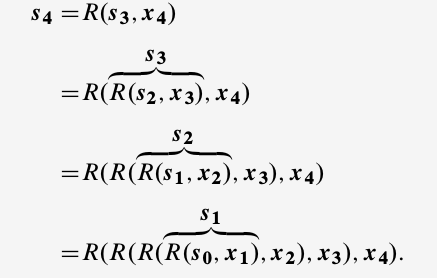
\includegraphics[scale = 0.35]{pics/RNN-recursion.png}
        \end{figure}
\item Thus, $\vec{s}_n$ and $\vec{y}_n$ can be thought of as encoding the entire input sequence.
\item The job of the network training is to set the parameters of $R$ and $O$ such that the state conveys useful information for the task we are tying to solve.

\end{itemize}
\end{scriptsize}
\end{frame}


\begin{frame}{RNN Training}
\begin{scriptsize}
\begin{itemize}
\item An unrolled RNN is just a very deep neural network.
\item The same parameters are shared across many parts of the computation.
\item Additional input is added at various layers.
\item To train an RNN network, need to create the unrolled computation graph for a given input sequence, add a loss node to the unrolled graph.
\item Then use the backward (backpropagation) algorithm to compute the gradients with respect to that loss.
\end{itemize}
\end{scriptsize}
\end{frame}

\begin{frame}{RNN Training}
\begin{scriptsize}
\begin{itemize}
\item This procedure is referred to in the RNN literature as backpropagation through time (BPTT).
\item The RNN does not do much on its own, but serves as a trainable component in a larger network.
\item The final prediction and loss computation are performed by that larger network, and the error is back-propagated through the RNN.
\item This way, the RNN learns to encode properties of the input sequences that are
useful for the further prediction task.
\item The supervision signal is not applied to the RNN directly, but through the larger network.
\end{itemize}
\end{scriptsize}
\end{frame}





\begin{frame}{Bidirectional RNNS (BIRNN)}
\begin{scriptsize}
\begin{itemize}
\item A useful elaboration of an RNN is a bidirectional-RNN (also commonly referred to as biRNN)
\item Consider the task of sequence tagging over a sentence.
\item An RNN allows us to compute a function of the $i$-th word $x_i$ based on the
past words $x_{1:i}$ up to and including it. 
\item However, the following words $x_{i+1:n}$ may also be useful for prediction,
\item The biRNN allows us to look arbitrarily far at both the past and the future within the sequence.
\end{itemize}
\end{scriptsize}
\end{frame}



\begin{frame}{Bidirectional RNNS (BIRNN)}
\begin{scriptsize}
\begin{itemize}
\item Consider an input sequence $\vec{x}_{1:n}$ . 
\item The biRNN works by maintaining two separate states, $s_{i}^{f}$ and $s_{i}^{b}$ for each input position $i$. 
\item The forward state $s_{i}^{f}$ is based on $\vec{x}_1, \vec{x}_2, \dots ,\vec{x}_i$, while the backward state $s_{i}^{b}$ is based on $\vec{x}_n, \vec{x}_{n-1}, \dots ,\vec{x}_i$.
\item The forward and backward states are generated
by two different RNNs.
\item The first RNN$(R^f, O^f)$  is fed the input sequence  $\vec{x}_{1:n}$ as is, while the second RNN$(R^b , O^b)$ is fed the input sequence in reverse.
\item The state representation $\vec{s}_i$ is then composed of both the forward and backward states.
\end{itemize}
\end{scriptsize}
\end{frame}


\begin{frame}{Bidirectional RNNS (BIRNN)}
\begin{scriptsize}
\begin{itemize}
\item The output at position $i$ is based on the concatenation of the two output vectors:
\begin{displaymath}
\vec{y}_i = [\vec{y}_{i}^{f};\vec{y}_{i}^{b}]=[O^{f}(s_{i}^{f});O^{b}(s_{i}^{b})
]
\end{displaymath}
\item The output takes into account both the past and the future.
\item The biRNN encoding of the $i$th word in a sequence is the concatenation of two RNNs, one reading the sequence from the beginning, and the other reading it from the end.
\item We define $biRNN(\vec{x}_{1:n}, i)$ to be the output vector corresponding to the $i$th sequence position:
\begin{displaymath}
biRNN(\vec{x}_{1:n}, i) = \vec{y}_i = [RNN^{f}(\vec{x}_{1:n});RNN^{b}(\vec{x}_{n:i})
\end{displaymath}
\end{itemize}
\end{scriptsize}
\end{frame}


\begin{frame}{Bidirectional RNNS (BIRNN)}
\begin{scriptsize}
\begin{itemize}
\item The vector $\vec{y}_i$ can then be used directly for prediction, or fed as part of the input to a more complex network.
\item While the two RNNs are run independently of each other, the error gradients
at position i will flow both forward and backward through the two RNNs.
\item Feeding the vector $\vec{y}_i$ through an MLP prior to prediction will further mix the forward and backward signals.
  \begin{figure}[h]
        	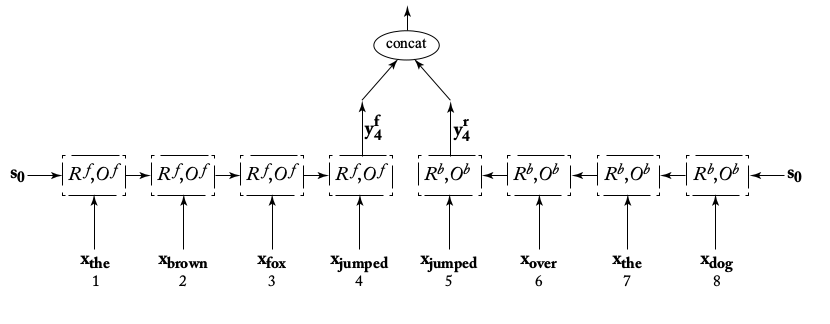
\includegraphics[scale = 0.35]{pics/biRNN.png}
        \end{figure}

\item Note how the vector $\vec{y}_4$ , corresponding to the word \textbf{jumped}, encodes an infinite window around (and including) the focus vector $\vec{x}_{jumped}$.        
\end{itemize}
\end{scriptsize}
\end{frame}


\begin{frame}{Bidirectional RNNS (BIRNN)}
\begin{scriptsize}
\begin{itemize}
\item Similarly to the $RNN$ case, we also define $biRNN^{*}(\vec{x}_{1:n})$ as the sequence of vectors $\vec{y}_{1:n}$:    
\begin{displaymath}
biRNN^{*}(\vec{x}_{1:n})= \vec{y}_{1:n} = biRNN(\vec{x}_{1:n},1),\dots,biRNN(\vec{x}_{1:n},n)
\end{displaymath}
\item The $n$ output vectors $\vec{y}_{1:n}$ can be efficiently computed in linear time by first running the forward and backward RNNs, and then concatenating the relevant outputs.
\end{itemize}
\end{scriptsize}
\end{frame}


\begin{frame}{Bidirectional RNNS (BIRNN)}
\begin{scriptsize}

  \begin{figure}[h]
        	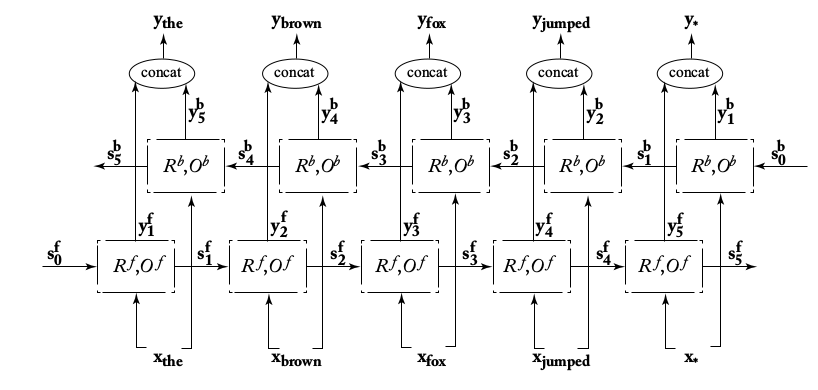
\includegraphics[scale = 0.35]{pics/biRNNstar.png}
        \end{figure}


\begin{itemize}

\item The biRNN is very effective for tagging tasks, in which each input vector corresponds to one output vector.

\item It is also useful as a general-purpose trainable feature-extracting component, that can be used whenever a window around a given word is required.
\end{itemize}
\end{scriptsize}
\end{frame}


\begin{frame}{Multi-layer (stacked) RNNS}
\begin{scriptsize}
\begin{itemize}
\item RNNs can be stacked in layers, forming a grid.
\item Consider $k$ RNNs, $RNN_{1},\dots, RNN_{k}$, where the $j$th RNN has states $\vec{s}_{1:n}^{j}$  and outputs $\vec{y}_{1:n}^{j}$.
\item The input for the first RNN are $\vec{x}_{1:n}$.
\item The input of the $j$th RNN ($j\geq 2$) are the outputs of the RNN below it, $\vec{y}_{1:n}^{j-1}$.
\item The output of the entire formation is the output of the last RNN, $\vec{y}_{1:n}^k$.
\item Such layered architectures are often called deep RNNs.
\end{itemize}
\end{scriptsize}
\end{frame}


\begin{frame}{Multi-layer (stacked) RNNS}
\begin{scriptsize}
  \begin{figure}[h]
        	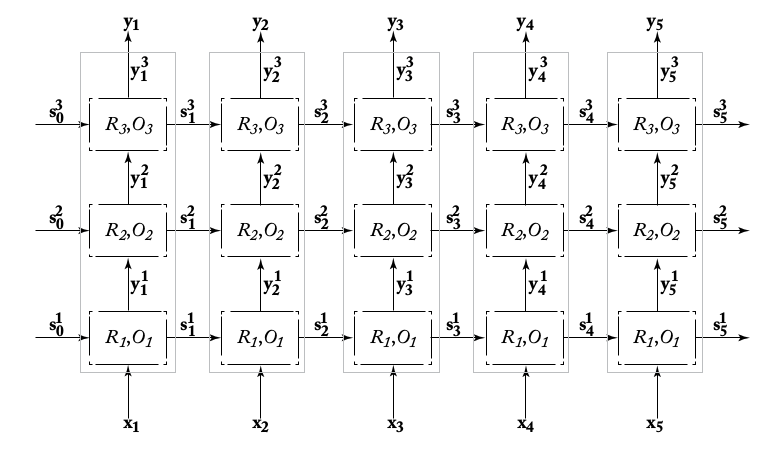
\includegraphics[scale = 0.35]{pics/stackedRNN.png}
        \end{figure}
\begin{itemize}
\item It is not theoretically clear what is the additional power gained by the deeper architecture.
\item It was observed empirically that deep RNNs work better than shallower ones on some tasks (e.g., machine translation).
\end{itemize}
\end{scriptsize}
\end{frame}


\begin{frame}{Elman Network or Simple-RNN}
\begin{scriptsize}
\begin{itemize}
\item After describing the RNN abstraction, we are now in place to discuss specific instantiations of it.
\item Recall that we are interested in a recursive function $\vec{s}_i =  R(\vec{x}_i, \vec{s}_{i-1})$ such that $\vec{s}_i$ encodes the sequence $\vec{x}_{1:n}$.
\item The simplest RNN formulation is known as an Elman Network or Simple-RNN (S-RNN).
\end{itemize}
\end{scriptsize}
\end{frame}

\begin{frame}{Elman Network or Simple-RNN}
\begin{scriptsize}
\begin{equation}
\begin{split}
\vec{s}_i & = R_{SRNN}(\vec{x}_{i},\vec{s}_{i-1}) = g(\vec{s}_{i-1}W^{s}+\vec{x}_{i}W^{x}+\vec{b}) \\
\vec{y}_i & = O_{SRNN}(\vec{s}_i) = \vec{s}_i \\
\vec{s}_i, \vec{y}_i \in  \mathcal{R}^{d_{s}}, & \quad  \vec{x}_i  \in \mathcal{R}^{d_{x}}, \quad W^{x} \in \mathcal{R}^{d_{x}\times d_{s}}, \quad W^{s} \in \mathcal{R}^{d_{s}\times d_{s}}, \vec{b} \in \mathcal{R}^{d_{s}} 
\end{split}
\end{equation}


\begin{itemize}
\item The state $\vec{s}_i$ and the input $\vec{x}_i$ are each linearly transformed.
\item The results are added (together with a bias term) and then passed through a nonlinear activation function g (commonly tanh or ReLU).
\item The Simple RNN provides strong results for sequence tagging as well as language modeling.
\end{itemize}
\end{scriptsize}
\end{frame}


\begin{frame}{Gated Architectures}
\begin{scriptsize}
\begin{itemize}
\item The S-RNN is hard to train effectively because of the \textbf{vanishing gradients} problem.
\item Error signals (gradients) in later steps in the sequence diminish quickly in the backpropagation process.
\item Thus, they do not reach earlier input signals, making it hard for the S-RNN to capture long-range dependencies.
\item Gating-based architectures, such as the LSTM [Hochreiter
and Schmidhuber, 1997] and the GRU [Cho et al., 2014b] are designed to solve this deficiency.
\end{itemize}
\end{scriptsize}
\end{frame}


\begin{frame}{Gated Architectures}
\begin{scriptsize}
\begin{itemize}
\item Consider the RNN as a general purpose computing device, where the state $\vec{s}_i$ represents a finite memory.
\item Each application of the function $R$ reads in an input $\vec{x}_{i+1}$ , reads in the current memory $\vec{s}_i$ , operates on them in some way, and writes the result into memory.
\item This resuls in a new memory state $\vec{s}_{i+1}$.
\item An apparent problem with the S-RNN architecture is that the memory access is not controlled. 
\item At each step of the computation, the entire memory state is read, and the entire memory state is written.
\end{itemize}
\end{scriptsize}
\end{frame}


\begin{frame}{Gated Architectures}
\begin{scriptsize}
\begin{itemize}
\item How does one provide more controlled memory access?
\item Consider a binary vector $\vec{g} \in {0,1}^n$. 
\item Such a vector can act as a \textbf{gate} for controlling access to $n$-dimensional vectors, using the hadamard-product operation $\vec{x} \odot \vec{g}$.
\item The hadamard operation is the same as the element-wise multiplication of two vectors:
\begin{displaymath}
\vec{x} = \vec{u} \odot \vec{v}  \Leftrightarrow  \vec{x}_{[i]} = \vec{u}_{[i]} \cdot \vec{v}_{[i]} \quad \forall i \in [1,n]
\end{displaymath}
\end{itemize}
\end{scriptsize}
\end{frame}




\begin{frame}{Gated Architectures}
\begin{scriptsize}
\begin{itemize}
\item Consider a memory $\vec{s} \in \mathcal{R}^{d}$, an input $\vec{x} \in \mathcal{R}^{d}$ and a gate $\vec{g} \in [0,1]^{d}$.
\item The following computation:
\begin{displaymath}
\vec{s}' \leftarrow \vec{g} \odot \vec{x} + (\vec{1}-\vec{g}) \odot (\vec{s}) 
\end{displaymath}
\item Reads the entries in $\vec{x}$ that correspond to the $\vec{1}$ values in $\vec{g}$ , and writes them to the new memory $\vec{s}'$.
\item Locations that weren't read to are copied from the memory $\vec{s}$ to the new memory $\vec{s}'$ through the use of the gate $(\vec{1}-\vec{g})$.
\end{itemize}
\end{scriptsize}
\end{frame}



\begin{frame}{Gated Architectures}
\begin{scriptsize}
  \begin{figure}[h]
        	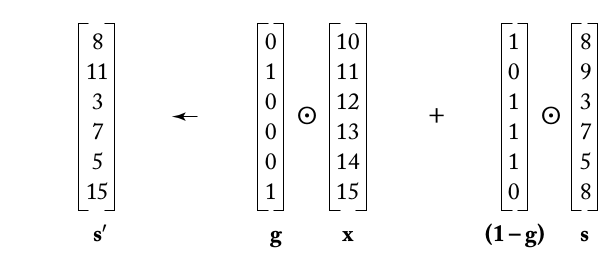
\includegraphics[scale = 0.35]{pics/gatedEx.png}
        \end{figure}
\begin{itemize}
\item This gating mechanism can serve as a building block in our RNN.
\item Gate vectors can be used to control access to the memory state $\vec{s}_i$.
\item We are still missing two important (and related) components: 
\begin{enumerate}
\begin{scriptsize}
 \item The gates should not be static, but be controlled by the
current memory state and the input.
\item Their behavior should be learned.
\end{scriptsize} 
\end{enumerate}
\item This introduced an obstacle, as learning in our framework entails being differentiable (because of the backpropagation algorithm).
\item The binary 0-1 values used in the gates are not differentiable.
\end{itemize}
\end{scriptsize}
\end{frame}


\begin{frame}{Gated Architectures}
\begin{scriptsize}

\begin{itemize}
\item A solution to this problem is to approximate the hard gating mechanism with a soft—but differentiable—gating mechanism.
\item To achieve these differentiable gates , we replace the requirement that $\vec{g} \in {0,1}^n$ and allow arbitrary real numbers, $\vec{g}' \in \mathcal{R}^n$.
\item These real numbers are then pass through a sigmoid function $\sigma(\vec{g}')$.
\item This bounds the value in the range $(0,1)$, with most values
near the borders.
\end{itemize}
\end{scriptsize}
\end{frame}



\begin{frame}{Gated Architectures}
\begin{scriptsize}

\begin{itemize}
\item When using the gate $\sigma(g')\odot \vec{x}$ , indices in $\vec{x}$ corresponding to near-one values in $\sigma(\vec{g}')$ are allowed to pass.
\item While those corresponding to near-zero values are blocked. 
\item The gate values can then be conditioned on the input and the current memory.
\item And can be trained using a gradient-based method to perform a desired behavior.
\item This controllable gating mechanism is the basis of the LSTM and the GRU architectures.
\item At each time step, differentiable gating mechanisms decide which parts of the inputs will be written to memory and which parts of memory will be overwritten (forgotten). 
\end{itemize}
\end{scriptsize}
\end{frame}


\begin{frame}{LSTM}
\begin{scriptsize}

\begin{itemize}
\item The Long Short-Term Memory (LSTM) architecture [Hochreiter and Schmidhuber, 1997] was designed to solve the vanishing gradients problem.
\item It was the the first architecture to introduce the gating mechanism.
\item The LSTM architecture explicitly splits the state vector $\vec{s}_i$ into two halves: 1) memory cells and 2) working memory.
\item The memory cells are designed to preserve the memory, and also the error gradients, across time, and are controlled through differentiable gating components\footnote{Smooth mathematical functions that simulate logical gates.}.
\item At each input state, a gate is used to decide how much of the new input should be written to the memory cell, and how much of the current content of the memory cell should be forgotten.
\end{itemize}
\end{scriptsize}
\end{frame}


\begin{frame}{LSTM}
\begin{scriptsize}

\begin{itemize}
\item Mathematically, the LSTM architecture is defined as:
  \begin{figure}[h]
        	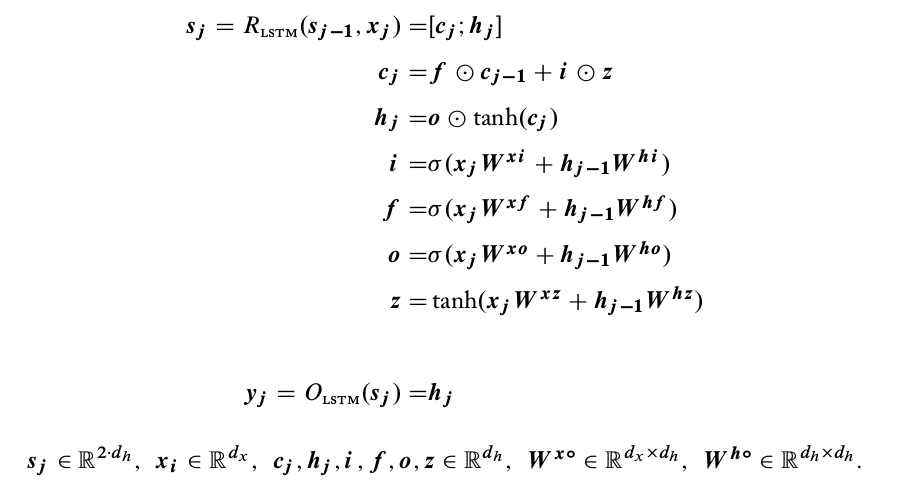
\includegraphics[scale = 0.35]{pics/LSTMform.png}
        \end{figure}
\end{itemize}
\end{scriptsize}
\end{frame}


\begin{frame}{LSTM}
\begin{scriptsize}

\begin{itemize}
\item The state at time $j$ is composed of two vectors, $\vec{c}_j$ and $h_{j}$, where $\vec{c}_j$ is the memory component and $\vec{h}_j$ is the hidden state component.
\item There are three gates, $\vec{i}$ , $\vec{f}$ , and $\vec{o}$, controlling for \textbf{i}nput, \textbf{f}orget, and \textbf{o}utput.
\item The gate values are computed based on linear combinations of the current input $\vec{x}_j$ and the previous state $\vec{h}_{j-1}$, passed through a sigmoid activation function.
\item An update candidate $\vec{z}$ is computed as a linear combination of $\vec{x}_j$ and $\vec{h}_{j-1}$ , passed through a tanh activation function (to push the values to be between -1 and 1).
\item The memory $\vec{c}_j$ is then updated: the forget gate controls how much of the previous memory to keep ($\vec{f} \odot \vec{c}_{j-1}$), and the input gate controls how much of the proposed update to keep ($\vec{i} \odot  \vec{z}$). 
\item Finally, the value of $\vec{h}_j$ (which is also the output $\vec{y}_j$ ) is determined based on the content of the memory $\vec{c}_j$ , passed through a tanh nonlinearity and controlled by the output gate. 
\item The gating mechanisms allow for gradients related to the memory part $\vec{c}_j$ to stay high across very long time ranges.
\end{itemize}
\end{scriptsize}
\end{frame}



\begin{frame}{LSTM}
  \begin{figure}[h]
        	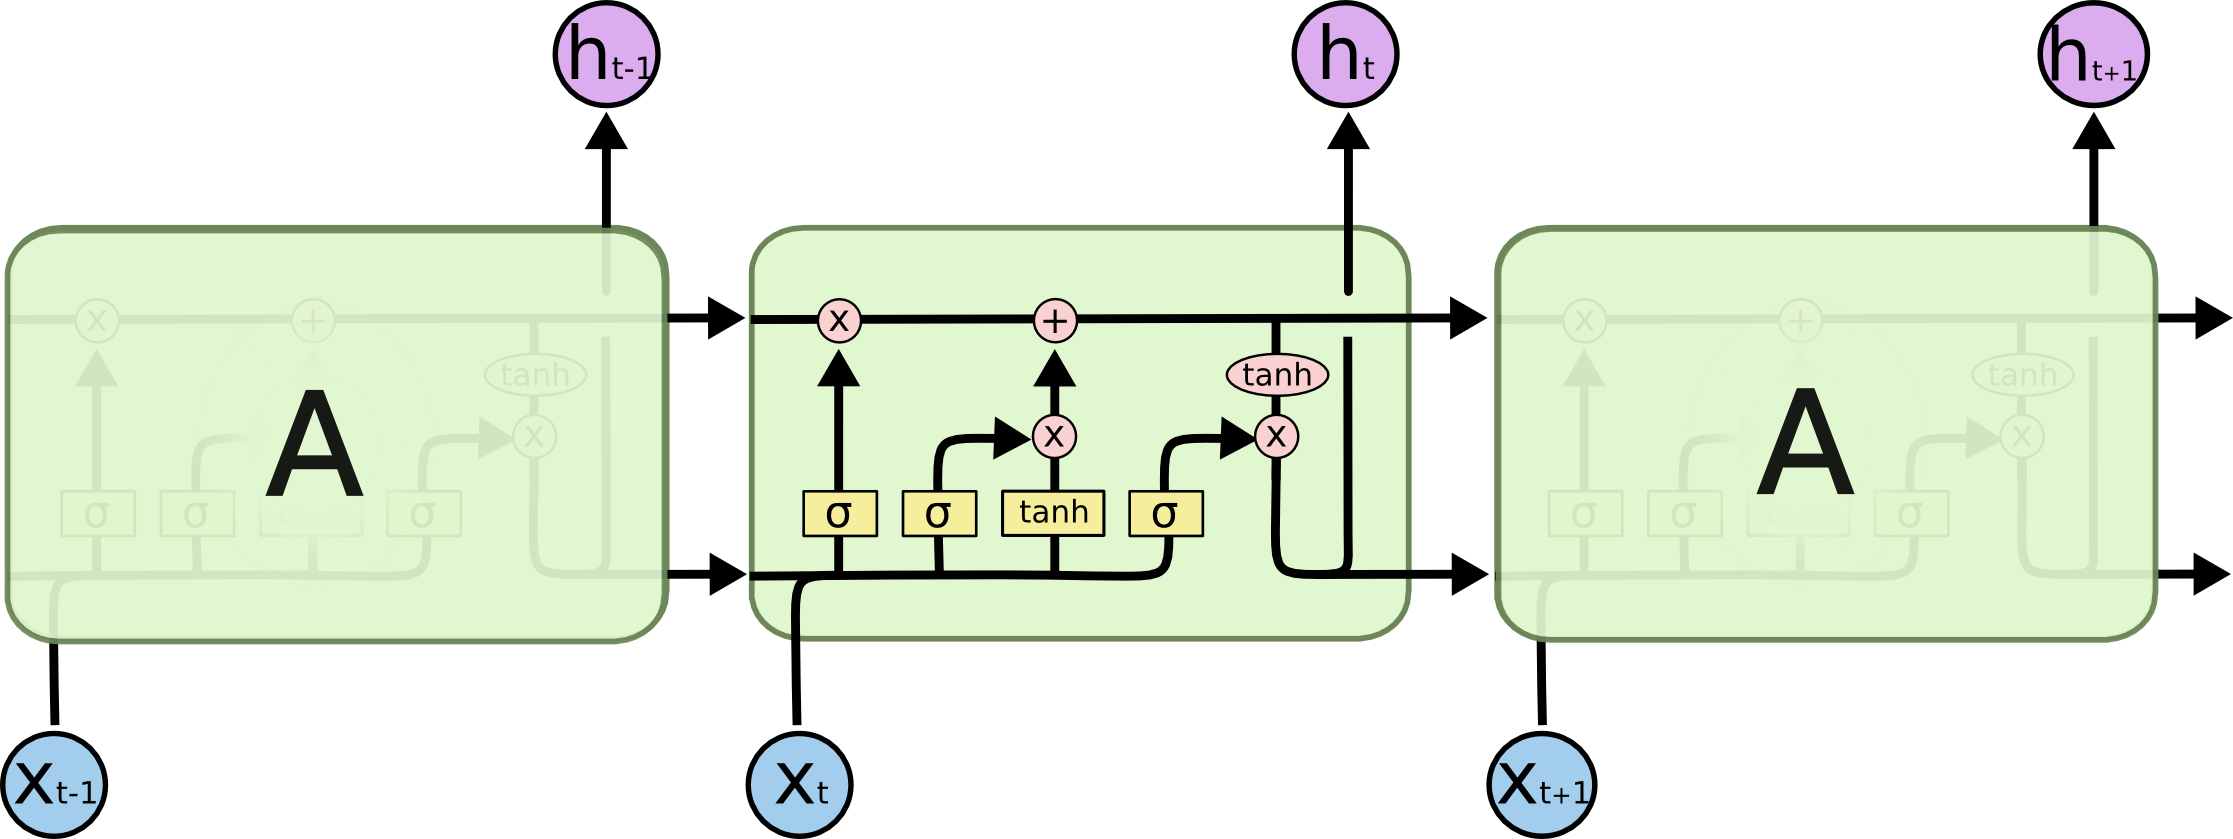
\includegraphics[scale = 0.35]{pics/LSTMchain.png}
        \end{figure}
\footnotemark{source: \url{http://colah.github.io/posts/2015-08-Understanding-LSTMs/}}        
\end{frame}


\begin{frame}{LSTM}
\begin{scriptsize}

\begin{itemize}
\item Intuitively, recurrent neural networks can be thought of as very deep feed-forward networks, with shared parameters across different layers.
\item For the Simple-RNN, the gradients then include repeated multiplication of the matrix $W$.
\item This makes the gradient values to vanish or explode.
\item The gating mechanism mitigate this problem to a large extent by getting rid of this repeated multiplication of a single matrix.
\item LSTMs are currently the most successful type of RNN architecture, and they are responsible for many state-of-the-art sequence modeling results.
\item The main competitor of the LSTM RNN is the GRU, to be discussed next.
\end{itemize}
\end{scriptsize}
\end{frame}



\begin{frame}{GRU}
\begin{scriptsize}

\begin{itemize}
\item The LSTM architecture is very effective, but also quite complicated.
\item The complexity of the system makes it hard to analyze, and also computationally expensive to work with.
\item The gated recurrent unit (GRU) was recently introduced by Cho et al. [2014b] as an alternative to the LSTM.
\item It was subsequently shown by Chung et al. [2014] to perform comparably to the LSTM on several (non textual) datasets.
\item Like the LSTM, the GRU is also based on a gating mechanism, but with substantially fewer gates and without a separate memory component.
\end{itemize}
\end{scriptsize}
\end{frame}



\begin{frame}{GRU}
  \begin{figure}[h]
        	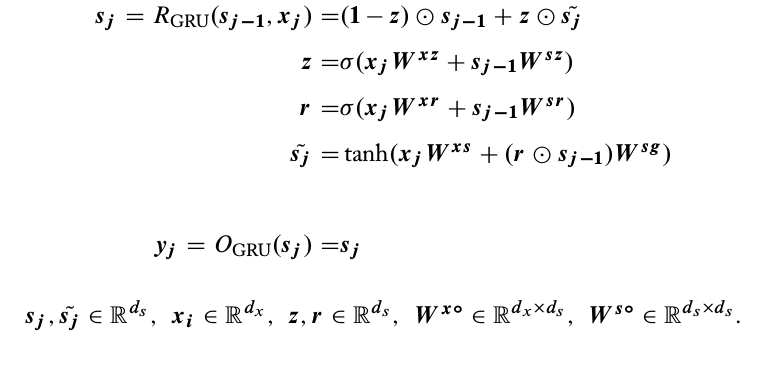
\includegraphics[scale = 0.35]{pics/GRU.png}
        \end{figure}        
\end{frame}



\begin{frame}{GRU}
\begin{scriptsize}
\begin{itemize}
\item One gate $\vec{r}$ is used to control access to the previous state $\vec{s}_{j-1}$ and compute a proposed update $\vec{\widetilde{s}}_j$.
\item The updated state $\vec{s}_j$ (which also serves as the output $\vec{y}_j$) is then determined based on an interpolation of the previous state $\vec{s}_{j-1}$ and the proposal $\vec{\widetilde{s}}_j$.
\item The proportions of the interpolation are controlled using the gate $\vec{z}$.
\item The GRU was shown to be effective in language modeling and machine translation.
\item However, the jury is still out between the GRU, the LSTM and possible alternative RNN architectures, and the subject is actively researched. 
\item For an empirical exploration of the GRU and the LSTM architectures, see Jozefowicz et al. [2015].
\end{itemize}
\end{scriptsize}
\end{frame}



\begin{frame}{Sentiment Classification with RNNs}
\begin{scriptsize}
\begin{itemize}
\item The simplest use of RNNs is as acceptors: read in an input sequence, and produce a binary or multi-class answer at the end.
\item RNNs are very strong sequence learners, and can pick-up on very
intricate patterns in the data.
\item An example of naturally occurring positive and negative sentences in the movie-reviews domain would be the following:
\item Positive: It's not life-affirming—it’s vulgar and mean, but I liked it.
\item Negative: It's a disappointing that it only manages to be decent instead of dead brilliant.
\end{itemize}
\end{scriptsize}
\end{frame}



\begin{frame}{Sentiment Classification with RNNs}
\begin{scriptsize}
\begin{itemize}
\item Note that the positive example contains some negative phrases (not life affirming, vulgar, and mean).
\item While the negative example contains some positive ones (dead brilliant).
\item Correctly predicting the sentiment requires understanding not only the individual phrases but also the context in which they occur, linguistic constructs such as negation, and the overall structure of the sentence.
\end{itemize}
\end{scriptsize}
\end{frame}

\begin{frame}{Sentiment Classification with RNNs}
\begin{scriptsize}
\begin{itemize}
\item The sentence-level sentiment classification task is modelled using an RNN-acceptor.
\item After tokenization, the RNN reads in the words of the sentence one at a time. \item The final RNN state is then fed into an MLP followed by a softmax-layer with two outputs (positive and negative). 
\item The network is trained with cross-entropy loss based on the gold sentiment labels.

\begin{equation}
\begin{split}
p(label = k | \vec{w}_{1:n}) & = \hat{\vec{y}}_{[k]} \\
\hat{\vec{y}} & = softmax(MLP(RNN(\vec{x}_{1:n}))) \\
\vec{x}_{1:n} & = E_{[w_{1}]}, \dots, E_{[w_{n}]} 
\end{split}
\end{equation}

\end{itemize}
\end{scriptsize}
\end{frame}




\begin{frame}{Sentiment Classification with RNNs}
\begin{scriptsize}
\begin{itemize}
\item The word embeddings matrix $E$ is initialized using pre-trained embeddings learned over a large external corpus using an algorithm such as word2vec or Glove with a relatively wide window.
\item It is often helpful to extend the model by considering bidirectional RNNs-
\item For longer sentences, Li et al. [2015] found it useful to use a hierarchical architecture, in which the sentence is split into smaller spans based on punctuation.
\item Then, each span is fed into a bidirectional RNN. 
\item Sequence of resulting vectors (onefor each span) are then fed into an RNN acceptor.
\item A similar hierarchical architecture was used for document-level sentiment classification in Tang et al. [2015].
\end{itemize}
\end{scriptsize}
\end{frame}

% https://arxiv.org/abs/1606.01781


\begin{frame}{Twitter Sentiment Classification with LSTMS Emojis}
\begin{scriptsize}
\begin{itemize}
\item An emoji-based distant supervision model for detecting sentiment and other affective states from short social media messages was proposed in \cite{FelboMSRL17}.
\item Emojis are used as a distant supervision approach for various affective detection tasks (e.g., emotion, sentiment, sarcasm) using a large corpus of 634M tweets with 64 emojis.
\item A neural network architecture is pretrained with this corpus. 
\item The network is an LSTM variant formed by an embedding layer, 2 bidrectional LSTM layers with normal skip connections and temporal average pooling-skip connections.
\end{itemize}
\end{scriptsize}
\end{frame}


\begin{frame}{DeepEmoji}
  \begin{figure}[h]
        	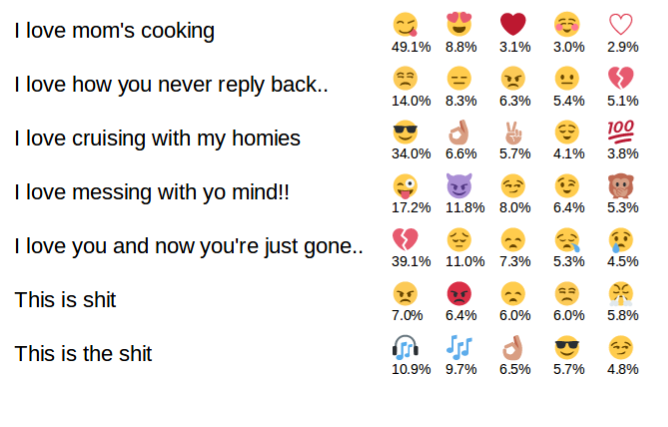
\includegraphics[scale = 0.45]{pics/deepEmoji1.png}
        \end{figure}    
        
\end{frame}




\begin{frame}{DeepEmoji}
   
    \begin{figure}[h]
        	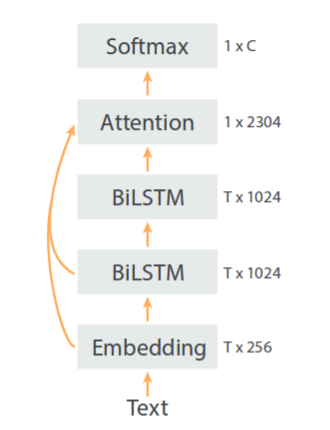
\includegraphics[scale = 0.45]{pics/deepEmoji2.png}
        \end{figure}       
        
\end{frame}




\begin{frame}{Twitter Sentiment Classification with LSTMS Emojis}
\begin{scriptsize}
\begin{itemize}
\item Authors propose the chain-thaw transfer-learning approach in which the pretrained network is fine-tuned for the target task. 
\item Here, each layer is individually fine-tuned in each step with the target gold data, and then they are all fine-tuned together. 
\item The model achieves state-of-the-art results the detection of emotion, sentiment, and sarcasm. 
\item  The pretrained network is released to the public.

\item  A demo of the model: \url{https://github.com/bfelbo/DeepMoji}.
\end{itemize}
\end{scriptsize}
\end{frame}


\begin{frame}{DeepEmoji}
        
         \begin{figure}[h]
        	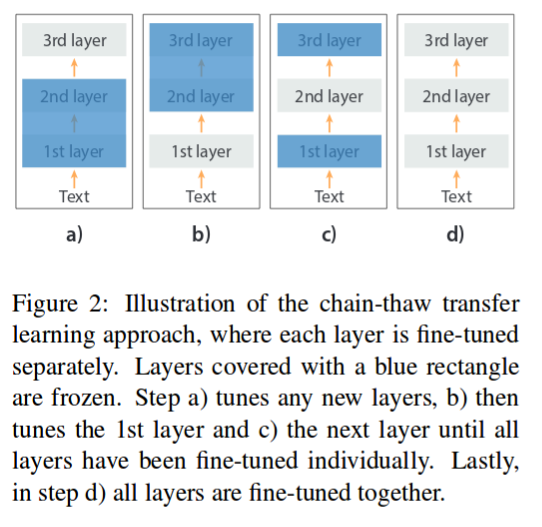
\includegraphics[scale = 0.45]{pics/deepEmoji3.png}
        \end{figure}        
        
\end{frame}







\begin{frame}{Recursive Neural Networks over Sentiment Treebank}
\begin{scriptsize}
\begin{itemize}
\item A recursive neural tensor network for learning the sentiment of pieces of texts of different granularities, such as words, phrases, and sentences, was proposed in~\cite{socher2013recursive}.
\item The network was trained on a sentiment annotated treebank \url{http://nlp.stanford.edu/sentiment/treebank.html} of parsed sentences for learning compositional vectors of words and phrases.
\item Every node in the parse tree receives a vector, and there is a matrix capturing how the meaning of adjacent nodes changes. 
\item The network is trained using a variation of backpropagation called Backprop through Structure.
\item The main drawback of this model is that it relies on parsing.
\end{itemize}
\end{scriptsize}
\end{frame}



\begin{frame}{Recursive Neural Networks over Sentiment Treebank}
   
    \begin{figure}[h]
        	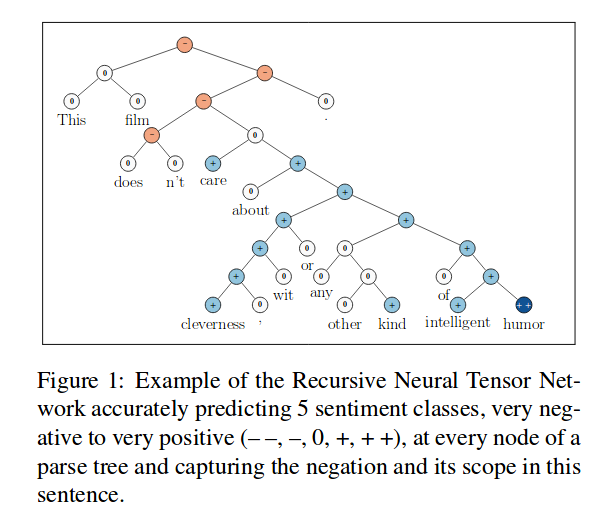
\includegraphics[scale = 0.45]{pics/recTensor1.png}
        \end{figure}       
        
\end{frame}


\begin{frame}{Recursive Neural Networks over Sentiment Treebank}
   
    \begin{figure}[h]
        	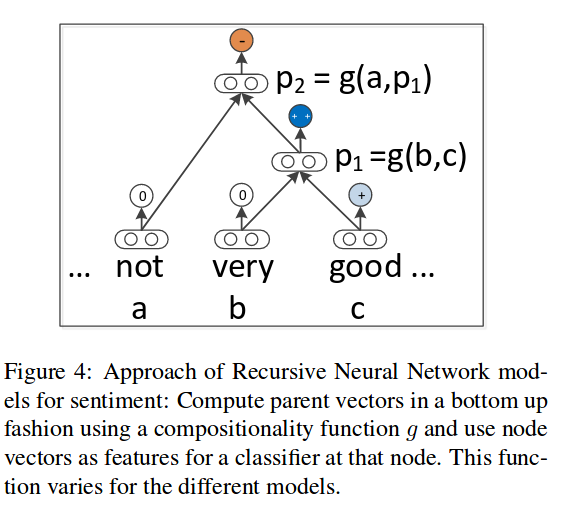
\includegraphics[scale = 0.45]{pics/recTensor2.png}
        \end{figure}       
        
\end{frame}



\begin{frame}{Paragraph vector}
% See dissapointment slide http://videolectures.net/deeplearning2015_manning_deep_learning/
\begin{scriptsize}
\begin{itemize}
\item A paragraph vector-embedding model that learns vectors for sequences of words of arbitrary length (e.g, sentences, paragraphs, or documents) without relying on parsing was proposed in~\cite{LeM14}. 
\item The paragraph vectors are obtained by training a similar network as the one used for training the CBOW embeddings. 
\item The words surrounding a centre word in a window are used as input together with a paragraph-level vector for predict the centre word. 
\item The paragraph-vector acts as a memory token that is used for all the centre words in the paragraph during the training the phase. 
\item The recursive neural tensor network and the paragraph-vector embedding were evaluated on the same movie review dataset used in \cite{Pang2002}, obtaining an accuracy of 85.4\% and 87.8\%, respectively. 
\item Both models outperformed the results obtained by classifiers trained on representations based on bag-of-words features.
\item Many researchers have have  struggled  to  reproduce these paragraph vectors \cite{lau2016empirical}.  
\end{itemize}
\end{scriptsize}
\end{frame}


\begin{frame}{Paragraph vector}
   
    \begin{figure}[h]
        	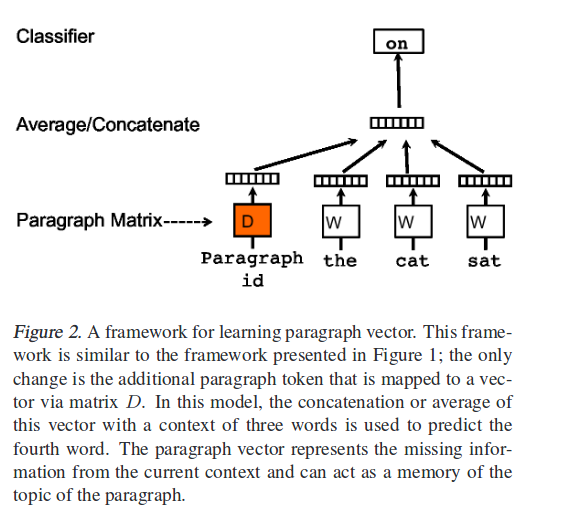
\includegraphics[scale = 0.45]{pics/doc2vec.png}
        \end{figure}       
        
\end{frame}


\begin{frame}{Summary}
\begin{scriptsize}
\begin{itemize}
\item Neural networks are making improvements across many NLP tasks (e.g., sentiment analysis).
\item Deep Learning $!=$ Feature Engineering.
\item Word embeddings provide a practical framework for semi-supervised learning (i.e., leveraging unlabelled data).
\item Character-level embeddings are worth paying attention to!
\item Convolutional neural networks can capture useful features (e.g., n-grams) regardless of the position.
\item Recurrent Neural Networks are very useful for learning temporal patterns, especially for long dependencies.
\item We just touched the surface!!
\end{itemize}
\end{scriptsize}


\end{frame}








\begin{frame}[allowframebreaks]\scriptsize
\frametitle{References}
\bibliography{../bio}
\bibliographystyle{apalike}
%\bibliographystyle{flexbib}
\end{frame}  


%%%%%%%%%%%%%%%%%%%%%%%%%%%

\end{document}
